\chapter{Desarrollo de la aplicación} % Main chapter title
\label{capitulo5} % Change X to a consecutive number; for referencing this chapter elsewhere, use \ref{capitulo6}
En este capítulo presentamos el proceso de desarrollo del módulo de gestión de programas orientado a competencias. Comenzamos listando las épicas y brindando una breve explicación de cada una de ellas.

La validación de las historias de usuario desarrolladas es de particular importancia. Si bien la validación se realizó de manera iterativa al final de los sprints, las presentamos en este escrito aparte, en el capítulo \ref{capitulo7}.

\subsection*{Épicas}
\begin{enumerate}
	\item Análisis de herramientas utilizadas y posibles potenciales para el desarrollo del módulo.
	\item Diseño de modelo de datos para versionamiento de competencias, cursos y programas.
	\item Desarrollo de flujo de trabajo para el versionamiento de competencias.
	\item Desarrollo de buzón de entrada para evaluadores y colaboradores del flujo de trabajo.
	\item Versionamiento encadenado de evaluaciones debido al versionamiento de competencias.
	\item Desarrollo de flujo de trabajo para el versionamiento de cursos.
	\item Desarrollo de flujo de trabajo para el versionamiento de programas de estudio.
 	\item Soporte de etapas en los flujos de trabajo.
	\item Desarrollo de reportes de versiones de cursos.
	\item Actualizar el AMS para que tome las versiones de competencias cursos y programas correspondientes en los periodos.
	\item Retoques finales.
\end{enumerate}

\resizebox{\columnwidth}{!}{%
\begin{ganttchart}[vgrid, hgrid, bar height=0.7, y unit chart=0.5cm, progress=today, today=24, bar label text={#1$\rightarrow$}, progress label text={#1$\%$}, today label=HOY]{1}{26}
\gantttitle{2016}{12}
\gantttitle{2017}{14} \ganttnewline
\gantttitle{Jul}{2}
\gantttitle{Ago}{2}
\gantttitle{Set}{2}
\gantttitle{Oct}{2}
\gantttitle{Nov}{2}
\gantttitle{Dic}{2}
\gantttitle{Ene}{2}
\gantttitle{Feb}{2}
\gantttitle{Mar}{2}
\gantttitle{Abr}{2}
\gantttitle{May}{2}
\gantttitle{Jun}{2} 
\gantttitle{Jul}{2} \\
\ganttbar[progress=100]{1}{1}{1} \\
\ganttbar[progress=100]{2}{2}{2} \\
\ganttbar[progress=100]{3}{3}{6} \\
\ganttbar[progress=100]{4}{5}{10} \\
\ganttbar[progress=100]{5}{11}{16} \\
\ganttbar[progress=100]{6}{11}{23} \\
\ganttbar[progress=100]{7}{13}{21} \\
\ganttbar[progress=100]{8}{23}{24} \\
\ganttbar[progress=100]{9}{22}{23} \\
\ganttbar[progress=100]{10}{22}{23} 
\end{ganttchart}
}


\section{Análisis de herramientas}
La primera etapa del proyecto fue realizar una encuesta a los posibles integrantes del nuevo equipo de desarrollo donde se verifican las capacidades adquiridas en cuanto a lenguajes de programación y tecnologías utilizadas, como así también de los conocimientos de dominio de la aplicación.
Dicha encuesta tiene como propósito permitir una mejor organización de los miembros de equipos y de esta manera una distribución eficaz de conocimientos y dominio de la aplicación para resolver las diferentes problemáticas que podría afectar al módulo currilar.
Una vez formado lo que sería el equipo de desarrollo se procedió a hacer análisis de las herramientas que podrían resolver la problemática entre ellas las que eran tomadas como requerimientos no funcionales para el módulo de gestión curricular del capítulo \ref{reqnofuncional}.
\section{Diseño de modelo de datos para versionamiento}
\subsection{Diseño del modelo de versionamiento para competencias, cursos y programas}
Al iniciar con las historias de versionamiento, se definió una tarea en la cual participaron algunos miembros de equipo y tenía como propósito principal el diseño de una lógica de negocios que permita adaptar las tablas existentes de las competencias, evaluaciones, cursos, y programas para que soporten una revisión o versionamiento de sus registros.

Como resúmen de actividades del modelo desarrollado (figura \ref{version_model}) se puede resaltar lo siguiente:
\begin{itemize}
	\item Cada tabla de cualquier entidad posee un identificador único. Las tablas entidades versionables son las de competencias, cursos, programas, y evaluaciones.
	\item Se decidió agregar una nueva columna \enquote{entity_atid} que tiene como propósito el de apuntar al origen de la versión. Por ejemplo; si el usuario crea un nuevo curso para el año lectivo, este curso tiene su identificador \enquote{course_id} y su \enquote{course_atid} apuntando a su mismo identificador por ser el origen para las versiones posteriores. Luego, se crea una nueva versión para el año posterior, esta nueva versión tiene su propio identificador pero su campo denominado como \enquote{course_atid} que apunta al primer curso creado u origen.
	\item Para hacer más sencilla la búsqueda de competencias, cursos, programas o evaluaciones actuales se agregó un campo a cada tabla identificando los actuales. Este campo denominado \enquote{is_current} o “es actual” es una bandera que indica la validez del registro.
	\item Además de registrar el origen, se registra la versión previa o de donde parte el registro con el campo \enquote{previous_entity_id}.
	\item Como cada registro de cualquier tabla ahora tiene un periodo de validez, se diseñaron tablas de relación entre cada tabla y la tabla de periodos lectivos denominada como \enquote{calendar}. Por ejemplo; \enquote{slo_term_rel} para las competencias, \enquote{new_course_term_rel} para los cursos, \enquote{asmt_term_rel} para las evaluaciones y \enquote{credential_term_rel} para los programas.
\end{itemize}

\begin{figure}
\centering
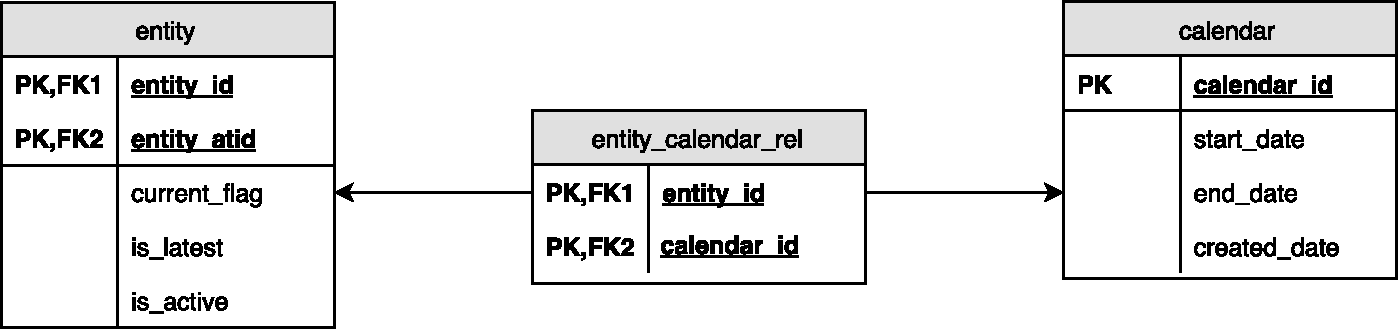
\includegraphics[width=125mm,scale=1]{Capitulos/DesarrollodelaAplicacion/Imagenes/version_model}
\caption{Modelo de datos para el versionamiento de competencias, cursos y programas.}
  \label{version_model}
\end{figure}
\section{Flujo de trabajo para el versionamiento de competencias}
\subsection{Versionamiento de competencias}
Esta historia de usuario tenía como descripción los siguiente \enquote{Como encargado del sistema de gestión de competencias, me gustaría ser capaz de versionar competencias con la finalidad de que se puedan redefinir competencias con el paso del tiempo, sin perder datos de corrección de las mismas}.

Algunas tareas que se definieron en la historia de usuario son las siguientes:
\begin{itemize}
	\item Investigar y diseñar el versionamiento de las competencias. La misma fue desarrollada de manera en que toda competencia versionada apunta al origen y el origen se apunta a sí mismo, de esta manera se puede saber la familia de versiones de una competencia.
	\item Actualizar todos esos lugares de la aplicación que listan las competencias, donde solamente deberían traer las competencias actuales.
	\item Manejar la distribución de competencias a periodos futuros, de manera que una competencia no pueda ser distribuida a periodos en las que no tiene validez.
	\item Diseñar y mantener pruebas automatizadas con Selenium.
\end{itemize}

Fue desarrollado durante tres iteraciones con un total de 170 horas cargadas en el sistema, debido a la complejidad a la hora de migrar los datos ya existentes de todas las universidades y por la cantidad de servicios que debían ser modificados.

\subsection{Flujo de trabajo simple}
En la siguiente historia de usuario inicia el proceso de creación de flujos de trabajo donde las plantillas de los flujos de trabajo pueden ser creados, editados y eliminados por el administrador encargado de la aplicación de cada universidad. Para esta historia se debe diseñar y desarrollar las plantillas de manera que el administrador pueda agregar los diferentes pasos del flujo de trabajo si así lo decide en el futuro. Inicialmente se considera un solo paso para la iteración inicial de desarrollo.

Esta historia de usuario tenía como descripción los siguiente \enquote{Como coordinador del AMS, me gustaría ser capaz de crear flujos de trabajo simples para administrar la aprobación de revisiones de competencias y que se pueda tener un mejor manejo de las creaciones y aprobaciones de las mismas en el campus}.

La historia tiene los siguientes criterios de aceptación:
\begin{itemize}
	\item Diseñar e implementar plantillas de flujo de trabajos simples para creación y revisión de todos los niveles de competencias.
	\item Diseñar e implementar un flujo de trabajo simple sin aprobación por parte de evaluadores, donde el iniciador del flujo puede revisar y aprobar su propio formulario.
	\item La plantilla de flujo de trabajo simple debe soportar el uso de pasos personalizados.
	\item El que inició el flujo es el único que puede llenar los campos del formulario.
\end{itemize}

El usuario debe ser capaz de agregar pasos personalizados para la plantilla de flujo de trabajo de la institución. Estos pasos personalizados son pasos que puede diseñar el usuario, donde puede colocar una pregunta como título y por cada título tiene un campo que puede llenar el usuario. Por lo general, un paso personalizado puede tener una o más preguntas definida por el usuario.

En los mockups entregados para el desarrollo se contemplan trabajos futuros donde cada paso tiene que ser aprobado por un rol del AMS, donde cualquier usuario con dicho rol puede aprobar o rechazar el flujo de trabajo con solo rechazar uno de los pasos. 

Además, se da inicio al desarrollo de plantillas de flujos de trabajo con las competencias, donde se podía asignar un tipo de flujo para cada plantilla ya sea de creación o versionamiento de los diferentes niveles de competencias.

Como las plantillas era una funcionalidad conocida y utilizada en otra parte de la aplicación, se imitó el comportamiento de la misma utilizando las mismas tablas para el almacenamiento de los datos en la base de datos relacional como requisito no funcional de la organización. Se diseñaron las nuevas pantallas con la definición de las plantillas de flujo de trabajo y también la pantalla para listar las mismas. En la misma el usuario administrador puede crear, editar si aún no ha sido usada, eliminar y clonar plantillas.

La historia de usuario fue desarrollada durante una iteración con un total de 90 horas cargadas en el sistema.

\subsection{Aprobación de pasos completados del flujo de trabajo para competencias}

Luego de la historia de diseño de las plantillas y un flujo de trabajo simple para creación o versionamiento de competencias, el siguiente paso es que un usuario designado desde la plantilla pueda iniciar y otro pueda aprobar el proceso de creación o revisión de competencias de cualquier nivel.

Esta historia de usuario tenía como descripción los siguiente \enquote{Como evaluador de un flujo de trabajo, me gustaría un simple proceso paso por paso para que pueda revisar y/o aprobar competencias de manera sencilla e intuitiva}.

La historia de usuario tiene los siguientes criterios de aceptación:
\begin{itemize}
	\item Soporte de asignaciones de tareas de creación y revisión por roles del AMS en las plantillas de flujos de trabajo.
	\item Diseño e implementación de vista de revisión para el flujo de trabajo.
\end{itemize}

Cada paso del flujo de trabajo debe estar terminado para que pase a la etapa de revisión por parte de los encargados. Luego de enviar el formulario, cada rol debe hacer su revisión para que el sistema pueda agregar la nueva competencia.

Como en las reuniones de demostración de cada sprint se notaban ciertos aspectos de las historias de usuario que no llenaban las expectativas de los clientes, los desarrolladores decidieron diseñar maquetas de pantallas que mostraban el posible diseño de la página. Luego de recibir feedback de parte de los clientes, se empezaba a desarrollar las nuevas pantallas. Finalizando la historia de usuario con pruebas automatizadas.

La historia de usuario fue desarrollada durante una iteración en un periodo de tiempo de 44 horas cargadas en el sistema.

\subsection{Rechazar pasos completados del flujo de trabajo}
Esta historia de usuario tenía como descripción los siguiente \enquote{Como evaluador de flujos de trabajo, me gustaría ser capaz de rechazar partes de los mismos y poder dar feedback a partes que no cumplen con nuestros estándares}.

\begin{itemize}
	\item Diseño e implementación de funcionalidad de rechazo de pasos en los flujos de trabajo.
	\item Diseño e implementación de funcionalidad de retroalimentación de parte de los evaluadores y encargados.
\end{itemize}

Esta funcionalidad tiene como propósito permitir a la persona que hace la revisión de los pasos rechazar y dejar feedback para que se puedan hacer los cambios correspondientes. Cuando se rechaza un paso, se rechaza el flujo de trabajo, y por lo tanto vuelven a estar activos los campos para que se hagan los cambios correspondientes.

El trabajo se inició la actualización del modelo de base de datos actual, luego de crear las clases correspondientes en el código para su utilización. Luego, se actualizaron las páginas donde el usuario puede aprobar los steps para que soporte rechazar pasos y poder así dejar algunos comentarios. 

La historia de usuario fue desarrollada durante una iteración en un periodo de tiempo de 53 horas cargadas en el sistema.

\section{Buzón de entrada para evaluadores y colaboradores del flujo de trabajo}
\subsection{Buzón de entradas de flujos de trabajo}
La siguiente historia tiene como propósito mostrar a cada usuario la lista de workflows pendientes que requiere de su aporte. Además de adaptar el nuevo buzón de entrada para otros rasgos de la aplicación como son las evaluaciones, los planes de acción y preguntas de parte del usuario a profesores.

Tiene como descripción lo siguiente \enquote{\textit{Como aprobador de eLumen, me gustaría una vista unificada de los workflows que tengo que revisar – además de mis evaluaciones, planes de acción y mis preguntas a profesores – para que no vaya cazando workflows por la aplicación}}

Como criterios de aceptación se encuentran los siguientes:
\begin{itemize}
	\item Diseño e implementación de buzón de entrada para flujos de trabajo.
	\item Diseño e implementación de buzón de entrada para planes de acción.
	\item Diseño e implementación de buzón de entrada para pedidos de profesores.
\end{itemize}

La historia fue finalizada en dos iteraciones con una cantidad de 56 horas cargadas en el sistema.

\subsection{Notificaciones con soporte a etapas}
La historia de usuario tiene como descripción lo siguiente \enquote{\textit{Como presidente curricular, me gustaría que el equipo de diseño y revisión curricular reciban notificaciones cuando tengan alertas de deuda de trabajo (y alertas cuando pase el tiempo), para que se puedan manejar mejor de esa manera los procesos curriculares}}.

Como criterios de aceptación se encuentran los siguientes:
\begin{itemize}
	\item Establecer notificaciones cuando las partes del flujo de trabajo son asignadas a los roles de las personas.
	\item Establecer notificaciones de alerta a asignaciones de partes y etapas. Por ejemplo, 5 días después de su asignación.
	\item Mandar notificaciones por mail.
\end{itemize}

Algunas de las tareas identificadas en la planificación de las iteraciones eran los siguientes:
\begin{itemize}
	\item Diseñar e implementar nuevos modelos de datos que permitan soportar el uso de roles para creadores y editores de partes.
	\item Actualizar el sistema de notificaciones del AMS.
	\item Diseñar e implementar la página de configuración de notificaciones.
\end{itemize}

La historia fue finalizada en tres iteraciones con una cantidad de 60 horas cargadas en el sistema.
\section{Versionamiento de evaluaciones}
La épica fue creada para abarcar todos los cambios que requerían las evaluaciones en sus diferentes formas de versionamiento. Entre ellas, se encuentra el versionamiento encadenado de las evaluaciones debido al flujo terminado de versionamiento de competencias. 

En caso de que existan evaluaciones ya creadas para las secciones de los cursos y en dicho curso se generaba una nueva versión de alguna de sus competencias, el sistema debía versionar las evaluaciones que utilizaba la versión anterior de dicha competencia con la versión actual para el periodo.

Como trabajo futuro se cuenta con el desarrollo de flujos de trabajo para las evaluaciones, ya que el versionamiento que ahora cuenta el sistema es automático y no a través de formularios web.

\begin{table}[H]
\centering
\resizebox{\columnwidth}{!}{%
\begin{tabular}{@{}lllll@{}}
\toprule
Historias de usuario           & HE & HC & PH &  Sprints \\ \midrule
Versionamiento de evaluaciones & 102 & 87 & 8 &  2 \\ \bottomrule
\end{tabular}
}
\caption{Historias de usuario para el versionamiento encadenado de evaluaciones debido al versionamiento de competencias}
\label{epic:5}
\end{table}

\subsection{Versionamiento de evaluaciones} \label{versionamiento_encadenado}
La historia de versionamiento de evaluaciones tiene como propósito permitir el versionamiento automático de evaluaciones existentes que utilizar competencias del sistema. Por ejemplo, en caso de que una evaluación hecha por un profesor tenga una nueva versión en el nuevo periodo de su sección, el sistema versiona la evaluación para ese periodo obteniendo las competencias actuales.

La historia de usuario tiene como descripción: \enquote{\textit{Como usuario del módulo curricular, me gustaría ser capaz de versionar mis evaluaciones, para que se observen los cambios a través del tiempo. Y que la interfaz y los reportes sigan presentando datos para los diseños históricos}}.

Algunas de las tareas fueron las siguientes:
\begin{itemize}
	\item Adaptar versionamiento para el modelo de datos de las evaluaciones.
	\item Migrar datos de los usuarios para que soporten versionamiento de las mismas.
	\item Actualizar el selector de evaluaciones de los profesores para que puedan seleccionar evaluaciones actuales.
	\item Actualizar el widget de profesores que utilizan las evaluaciones como datos.
\end{itemize}

Esta historia de usuario fue realizada en una iteración con un total de 87 horas cargadas en el sistema.

\section{Flujo de trabajo para el versionamiento de cursos}
\begin{table}[H]
\centering
\resizebox{\columnwidth}{!}{%
\begin{tabular}{@{}lllll@{}}
\toprule
Historias de usuario              & HE & HC & PH & Sprints \\ \midrule
Versionamiento de cursos          & 84 & 96 & 13 & 3       \\
Información básica de curso       & 46 & 53 & 5  & 1       \\
Horas y unidades de evaluación    & 48 & 66 & 5  & 1       \\
Especificaciones de curso         & 40 & 40 & 5  & 1       \\
Requisitos de curso               & 44 & 40 & 5  & 1       \\
Revisar y aprobar curso           & 48 & 68 & 5  & 1       \\
Competencias de curso             & 80 & 76 & 8  & 1       \\
Esquema de curso                  & 40 & 48 & 5  & 1       \\
Códigos de clasificación de curso & 56 & 80 & 5  & 1       \\ \bottomrule
\end{tabular}
}
\caption{Historias de usuario para el flujo de trabajo para el versionamiento de cursos}
\label{epic:6}
\end{table}


\subsection{Versionamiento de cursos}
Esta historia de usuario fue realizada en tres iteraciones con un total de 96 horas cargadas, debido a que los cambios que suponía conllevan a una migración importante de datos de los usuarios.

Tenía como descripción: \enquote{\textit{Como coordinador del AMS, me gustaría poder hacer una versión de mi plan de curso para que pueda realizar un seguimiento de los cambios para cosas como la revisión de programas y los acuerdos de articulación y transferencia en la aplicación}}.

Algunas de las tareas realizadas en la historia fueron las siguientes:

\begin{itemize}
	\item Buscar técnicas y herramientas de versionamiento parecidas para implementar.
	\item Diseñar una posible solución a la problemática.
	\item Implementar cambios en la base de datos mediante scripts en el proyecto.
	\item Actualizar clases Java existentes en el proyecto de cursos.
	\item Implementar la solución para el flujo de trabajo.
	\item Actualizar la creación de cursos sin el módulo curricular con los nuevos campos.
	\item Adaptar la relación de cursos y competencias para que soporte el versionamiento de los mismos.
	\item Actualizar la lista de competencias por cursos.
\end{itemize}

\subsection{Información básica de curso}
Esta historia de usuario tiene como propósito de diseñar páginas que permitan al usuario completar la información básica de curso que buscan diseñar, así también fueron proporcionados mockups para la pantalla (figura \ref{course_cover_info}).

Tiene la siguiente descripción: \enquote{\textit{Como miembro del comité de Curriculum, me gustaría ser capaz de administrar la página de información básica de cursos, para que no tenga que buscar por documentos a la hora de crear o versionar cursos}}.

\begin{itemize}
	\item Diseñar un modelo de datos que soporte el nuevo formato de información de curso.
	\item Adaptar tablas existentes y crear clases nuevas para las nuevas entidades de base de datos.
	\item Actualizar la plantilla de creación de Workflow para que soporte el nuevo paso.
	\item Actualizar el visualizador de Workflow.
	\item Diseño de pruebas automatizadas.
\end{itemize}

La historia se terminó en una iteración con un total de 53 horas de desarrollo.

\begin{figure}[H]
\centering
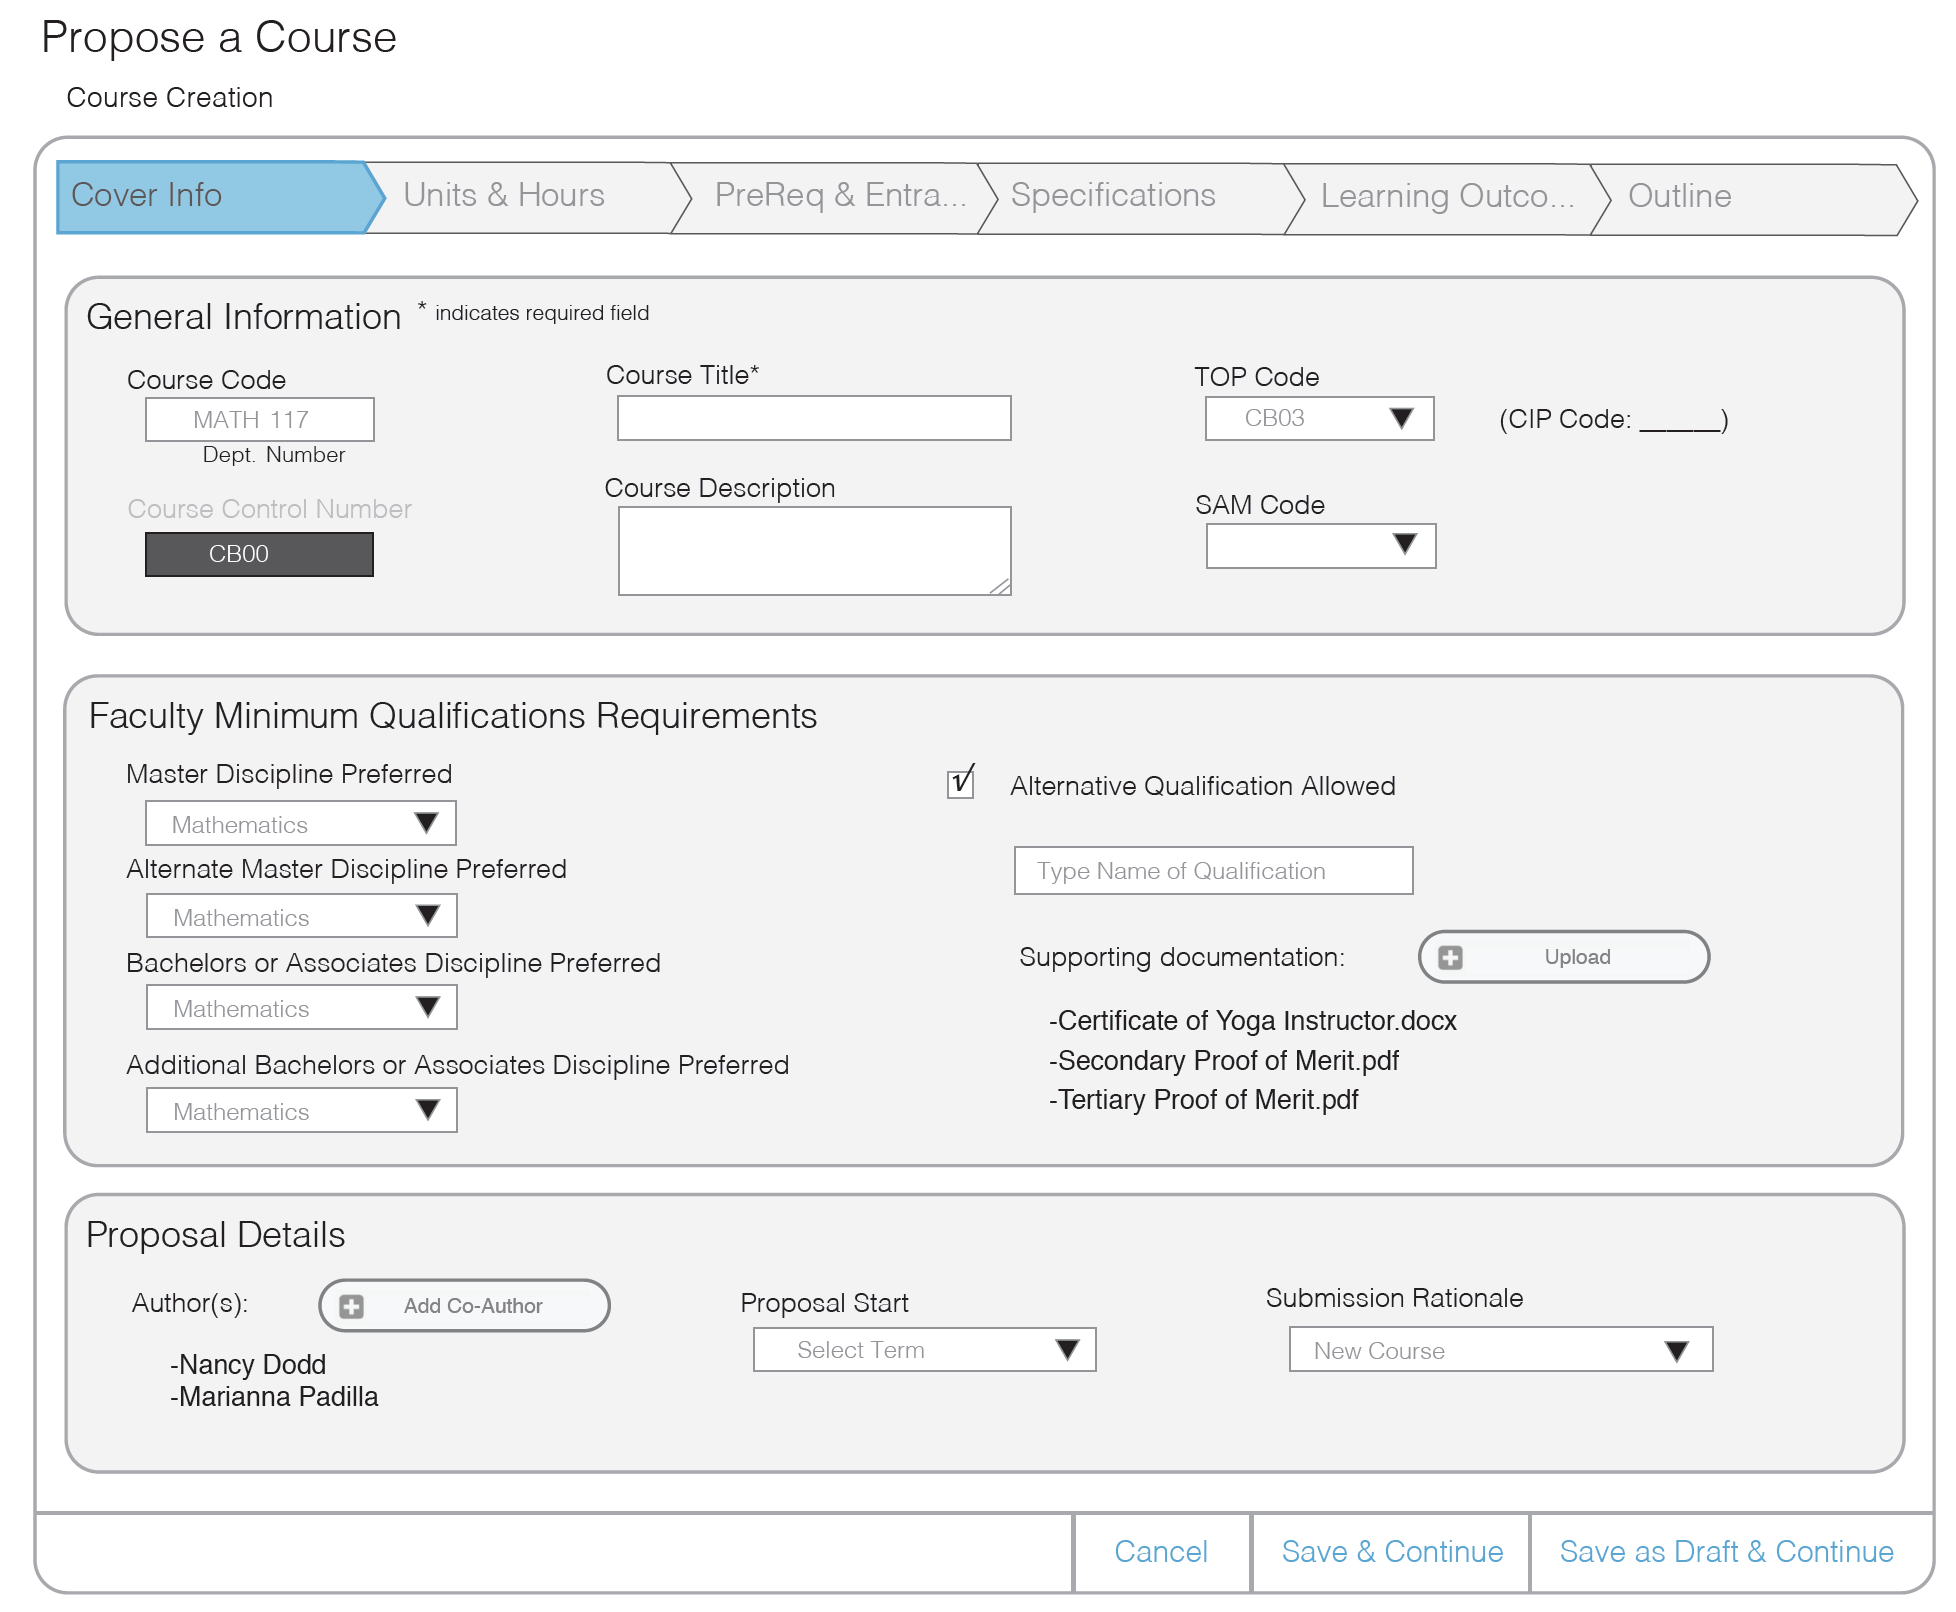
\includegraphics[scale=0.3]{Capitulos/DesarrollodelaAplicacion/Imagenes/course_cover_info}
\caption{Mockup de la pantalla de información básica de curso.}
  \label{course_cover_info}
\end{figure}

\subsection{Horas y unidades de evaluación}
En esta historia se desarrolló un nuevo paso para el desarrollo de flujo de trabajo, en la cual el encargo del mismo va a poder detallar las horas y unidades que requiere el curso o que va a requerir.

La organización ha proveído mockups (figura \ref{course_units_hours}) para la página como criterio de aceptación de la historia es que siga el modelo de la misma.

La historia tenía la siguiente descripción: \enquote{\textit{Como profesor encargado del curso, me gustaría tener una página de horas y métricas para que pueda conseguir información básica sobre mi curso en el AMS}}.

La historia a desarrollar se dividió entre miembros del equipo de desarrollo en las siguientes tareas:
\begin{itemize}
	\item Modificar el modelo de datos para que soporte los nuevos campos de curso.
	\item Crear y/o editar las clases Java.
	\item Actualizar la plantilla de flujo de trabajos.
	\item Actualizar el visualizador de flujo de trabajos.
	\item Pruebas de funcionalidad.
\end{itemize}

La historia ha sido terminada en una iteración con un total de 66 horas de desarrollo.

\begin{figure}[H]
\centering
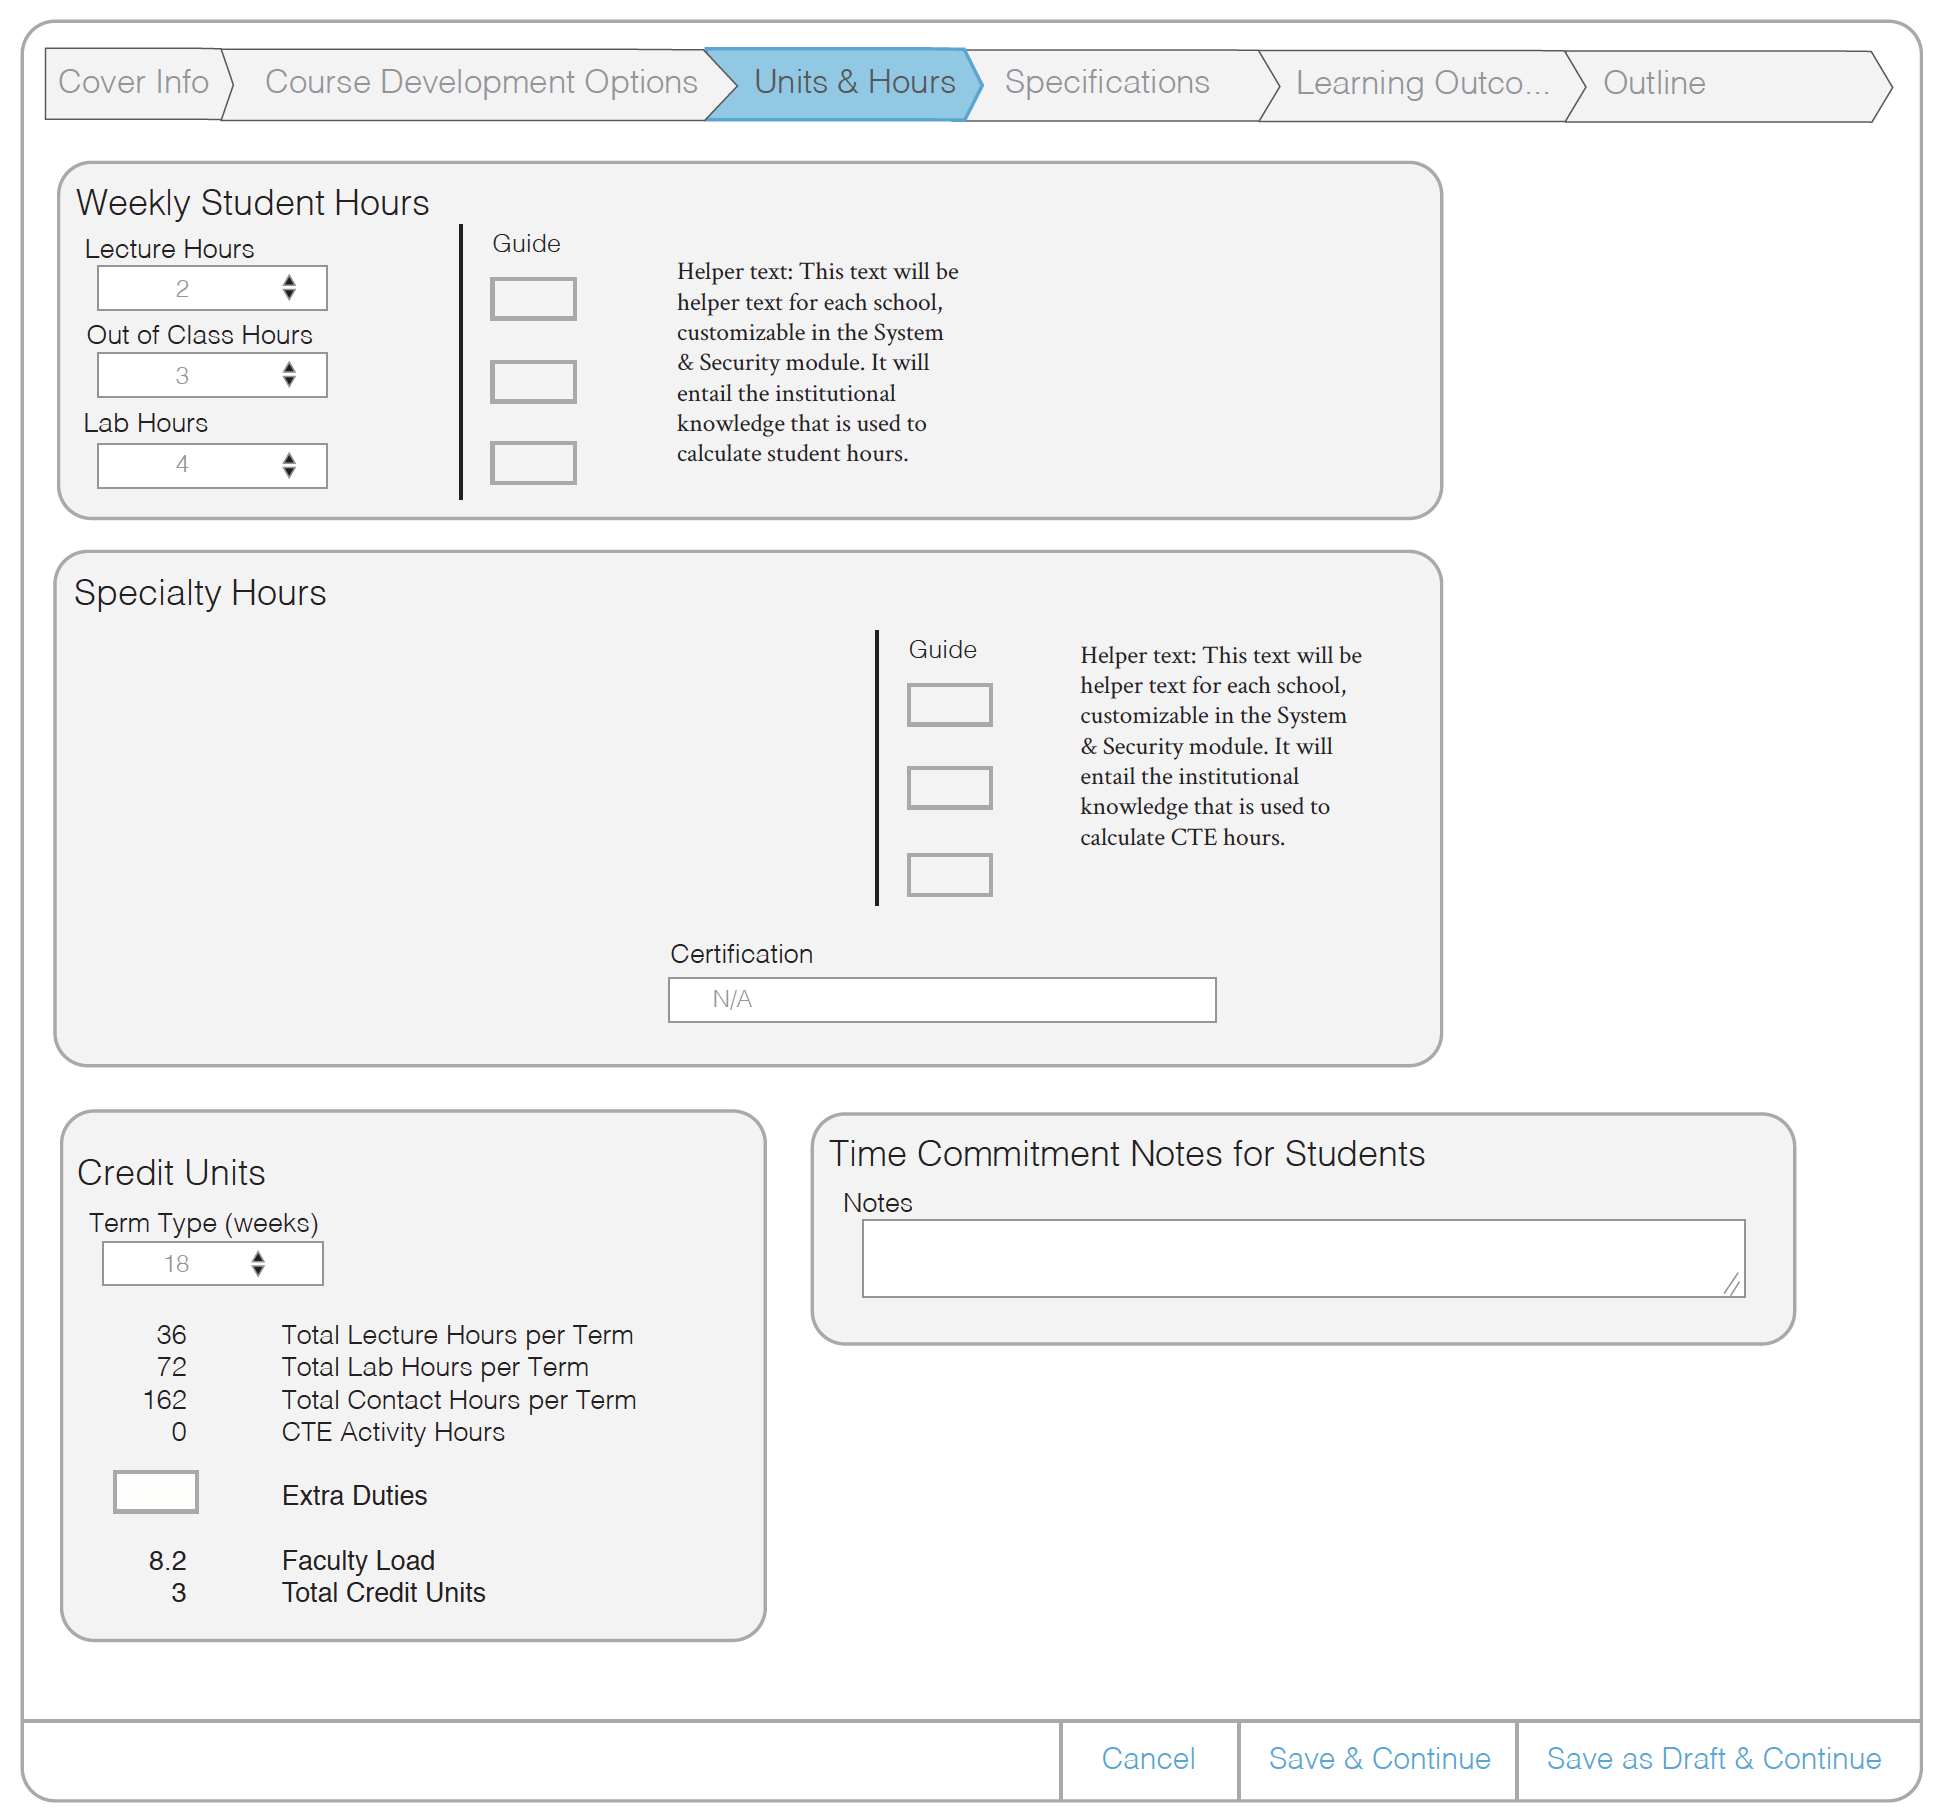
\includegraphics[scale=0.3]{Capitulos/DesarrollodelaAplicacion/Imagenes/course_units_hours}
\caption{Mockup de la pantalla de horas y unidades de evaluación de curso.}
  \label{course_units_hours}
\end{figure}

\subsection{Especificaciones de curso}
En la siguiente historia de usuario ha desarrollado un nuevo paso para el flujo de trabajo en la cual el encargado del flujo de trabajo puede agregar objetivos, información acerca de los métodos de evaluación de la materia, algunos equipos requeridos y libros que se necesitará en el curso.

Se han proporcionado de mockups (figura \ref{course_specs}) para el nuevo paso y era un criterio de aceptación de la historia de usuario seguir el mismo formato para el desarrollo de la misma.

La historia de usuario proporciona la siguiente descripción: \enquote{\textit{Como profesor encargado de curso, me gustaría ser capaz de agregar o editar especificaciones de curso como parte del flujo de trabajo de creación y/o versionamiento de mi curso para no tener que hacerlo en papel}}.

Las tareas fueron separadas y desarrolladas por los desarrolladores y eran las siguientes:
\begin{itemize}
	\item Migrar los datos para que soporte el nuevo formato de cursos.
	\item Crear y/o modificar clases de Java para el nuevo modelo de datos.
	\item Actualizar la página de plantillas de flujo de trabajo para que soporte el nuevo paso.
	\item Actualizar el visualizador de flujo de trabajo.
	\item Actualizar los servicios de guardado para creación y versionamiento de cursos y flujo de trabajos.
	\item Actualizar el servicio de aprobación de flujo de trabajo.
\end{itemize}

La historia fue terminada en una iteración con 40 horas de desarrollo cargadas en el sistema

\begin{figure}[H]
\centering
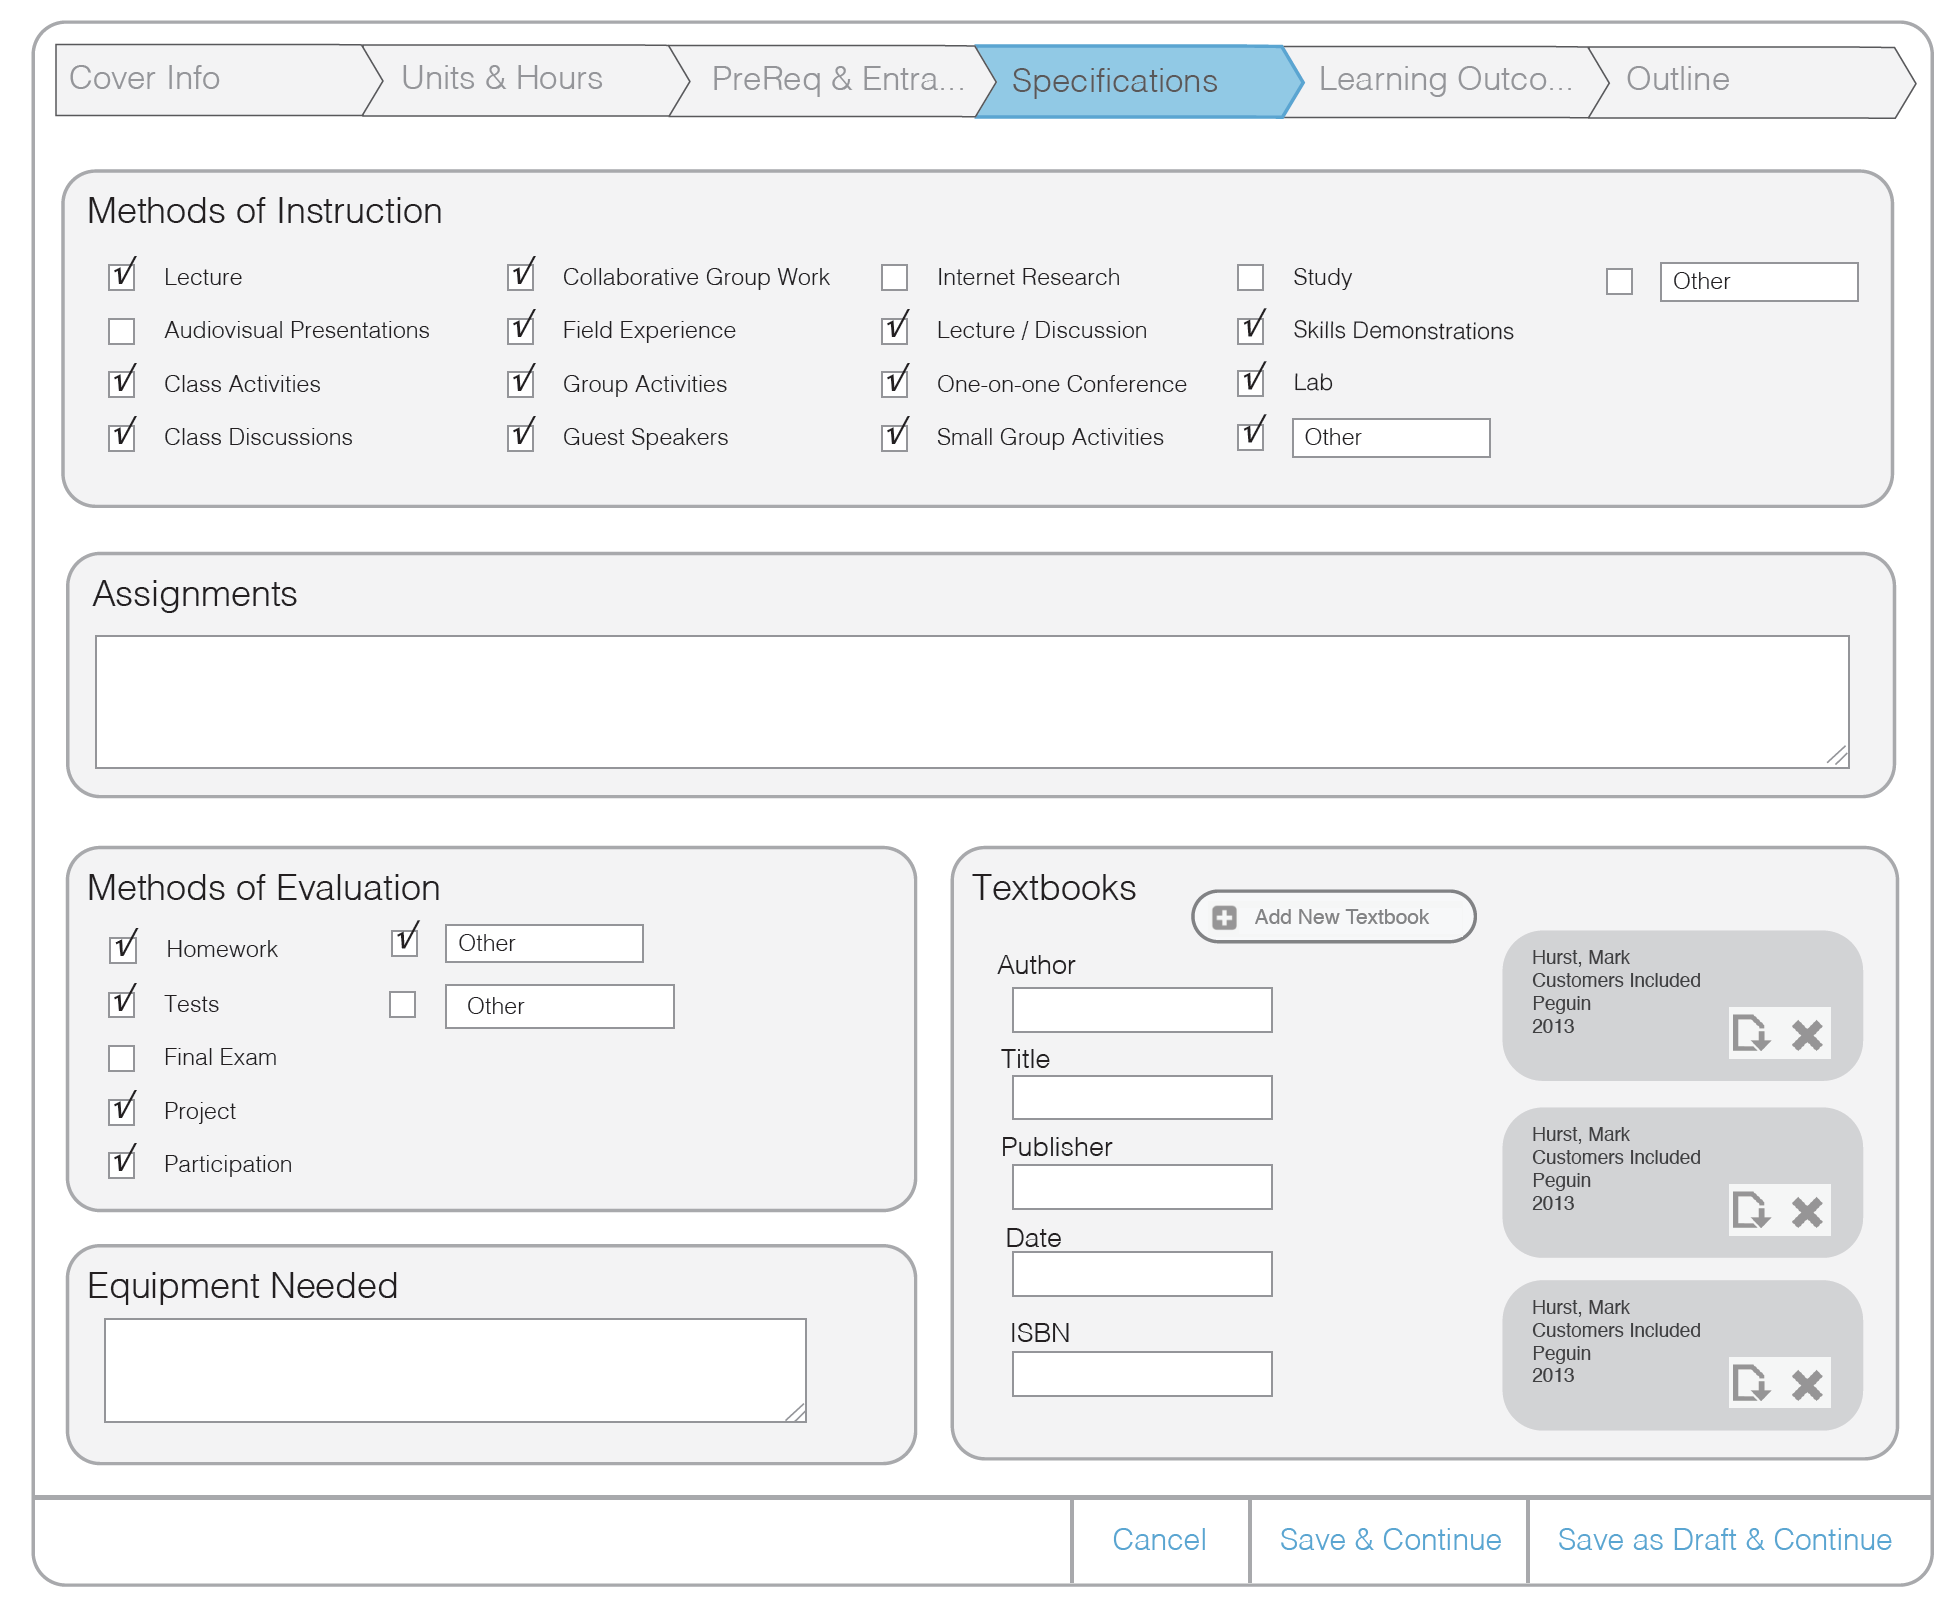
\includegraphics[scale=0.3]{Capitulos/DesarrollodelaAplicacion/Imagenes/course_specs}
\caption{Mockup de la pantalla de especificaciones de curso.}
  \label{course_specs}
\end{figure}

\subsection{Requisitos de curso}
Esta historia tiene como propósito el de adaptar el modelo de datos para que una lista de cursos como pre-requisitos, co-requisitos, anti-requisitos, y recomendaciones para su nuevo curso. Además, de ciertas capacidades que el alumno debe tener como requisito para tomar el curso.

Para entrar un poco en contexto de la historia vamos a definir cuáles son los tipos de requisitos que puede tener un curso:

\begin{itemize}
	\item \textbf{Pre-requisito:} es un tipo de requisito que impide al usuario tomar o cursar un curso sin haber aprobado antes del curso que está como pre-requisito.
	\item \textbf{Co-requisito:} es un tipo de requisito que impide al usuario tomar un curso si no cursa también el curso que tiene como co-requisito.
	\item \textbf{Anti-requisito:} es un requisito que impide al usuario tomar un curso si ya aprobó o va a tomar un curso que tiene como anti-requisito.
	\item \textbf{Recomendación:} es una recomendación por parte del sistema que materia tomar para aprovechar mejor la malla. Es opcional.
\end{itemize}

La historia de usuario tiene como descripción: \enquote{\textit{Como persona encargada de un curso, me gustaría ser capaz de introducir requisitos para cursos y ciertas competencias adquiridas en la creación o revisión de flujo de trabajo, para que podamos seguir durante su desarrollo y aprobación}} y la figura \ref{course_req} muestra mockups para la pantalla.

La historia fue dividida en partes para que los desarrolladores puedan trabajar en partes independientes durante el proceso de la misma, y eran las siguientes:
\begin{itemize}
	\item Diseñar y actualizar el modelo de datos actual.
	\item Generar y actualizar clases Java para la lógica.
	\item Actualizar la plantilla de flujo de trabajo para que soporte un nuevo paso.
	\item Actualizar el visualizador de flujo de trabajo.
	\item Actualizar los servicios de guardado y aprobación.
	\item Pruebas de funcionalidad.
\end{itemize}

La historia de usuario ha sido terminada en una iteración con 44 horas de desarrollo cargadas en el sistema.

\begin{figure}[H]
\centering
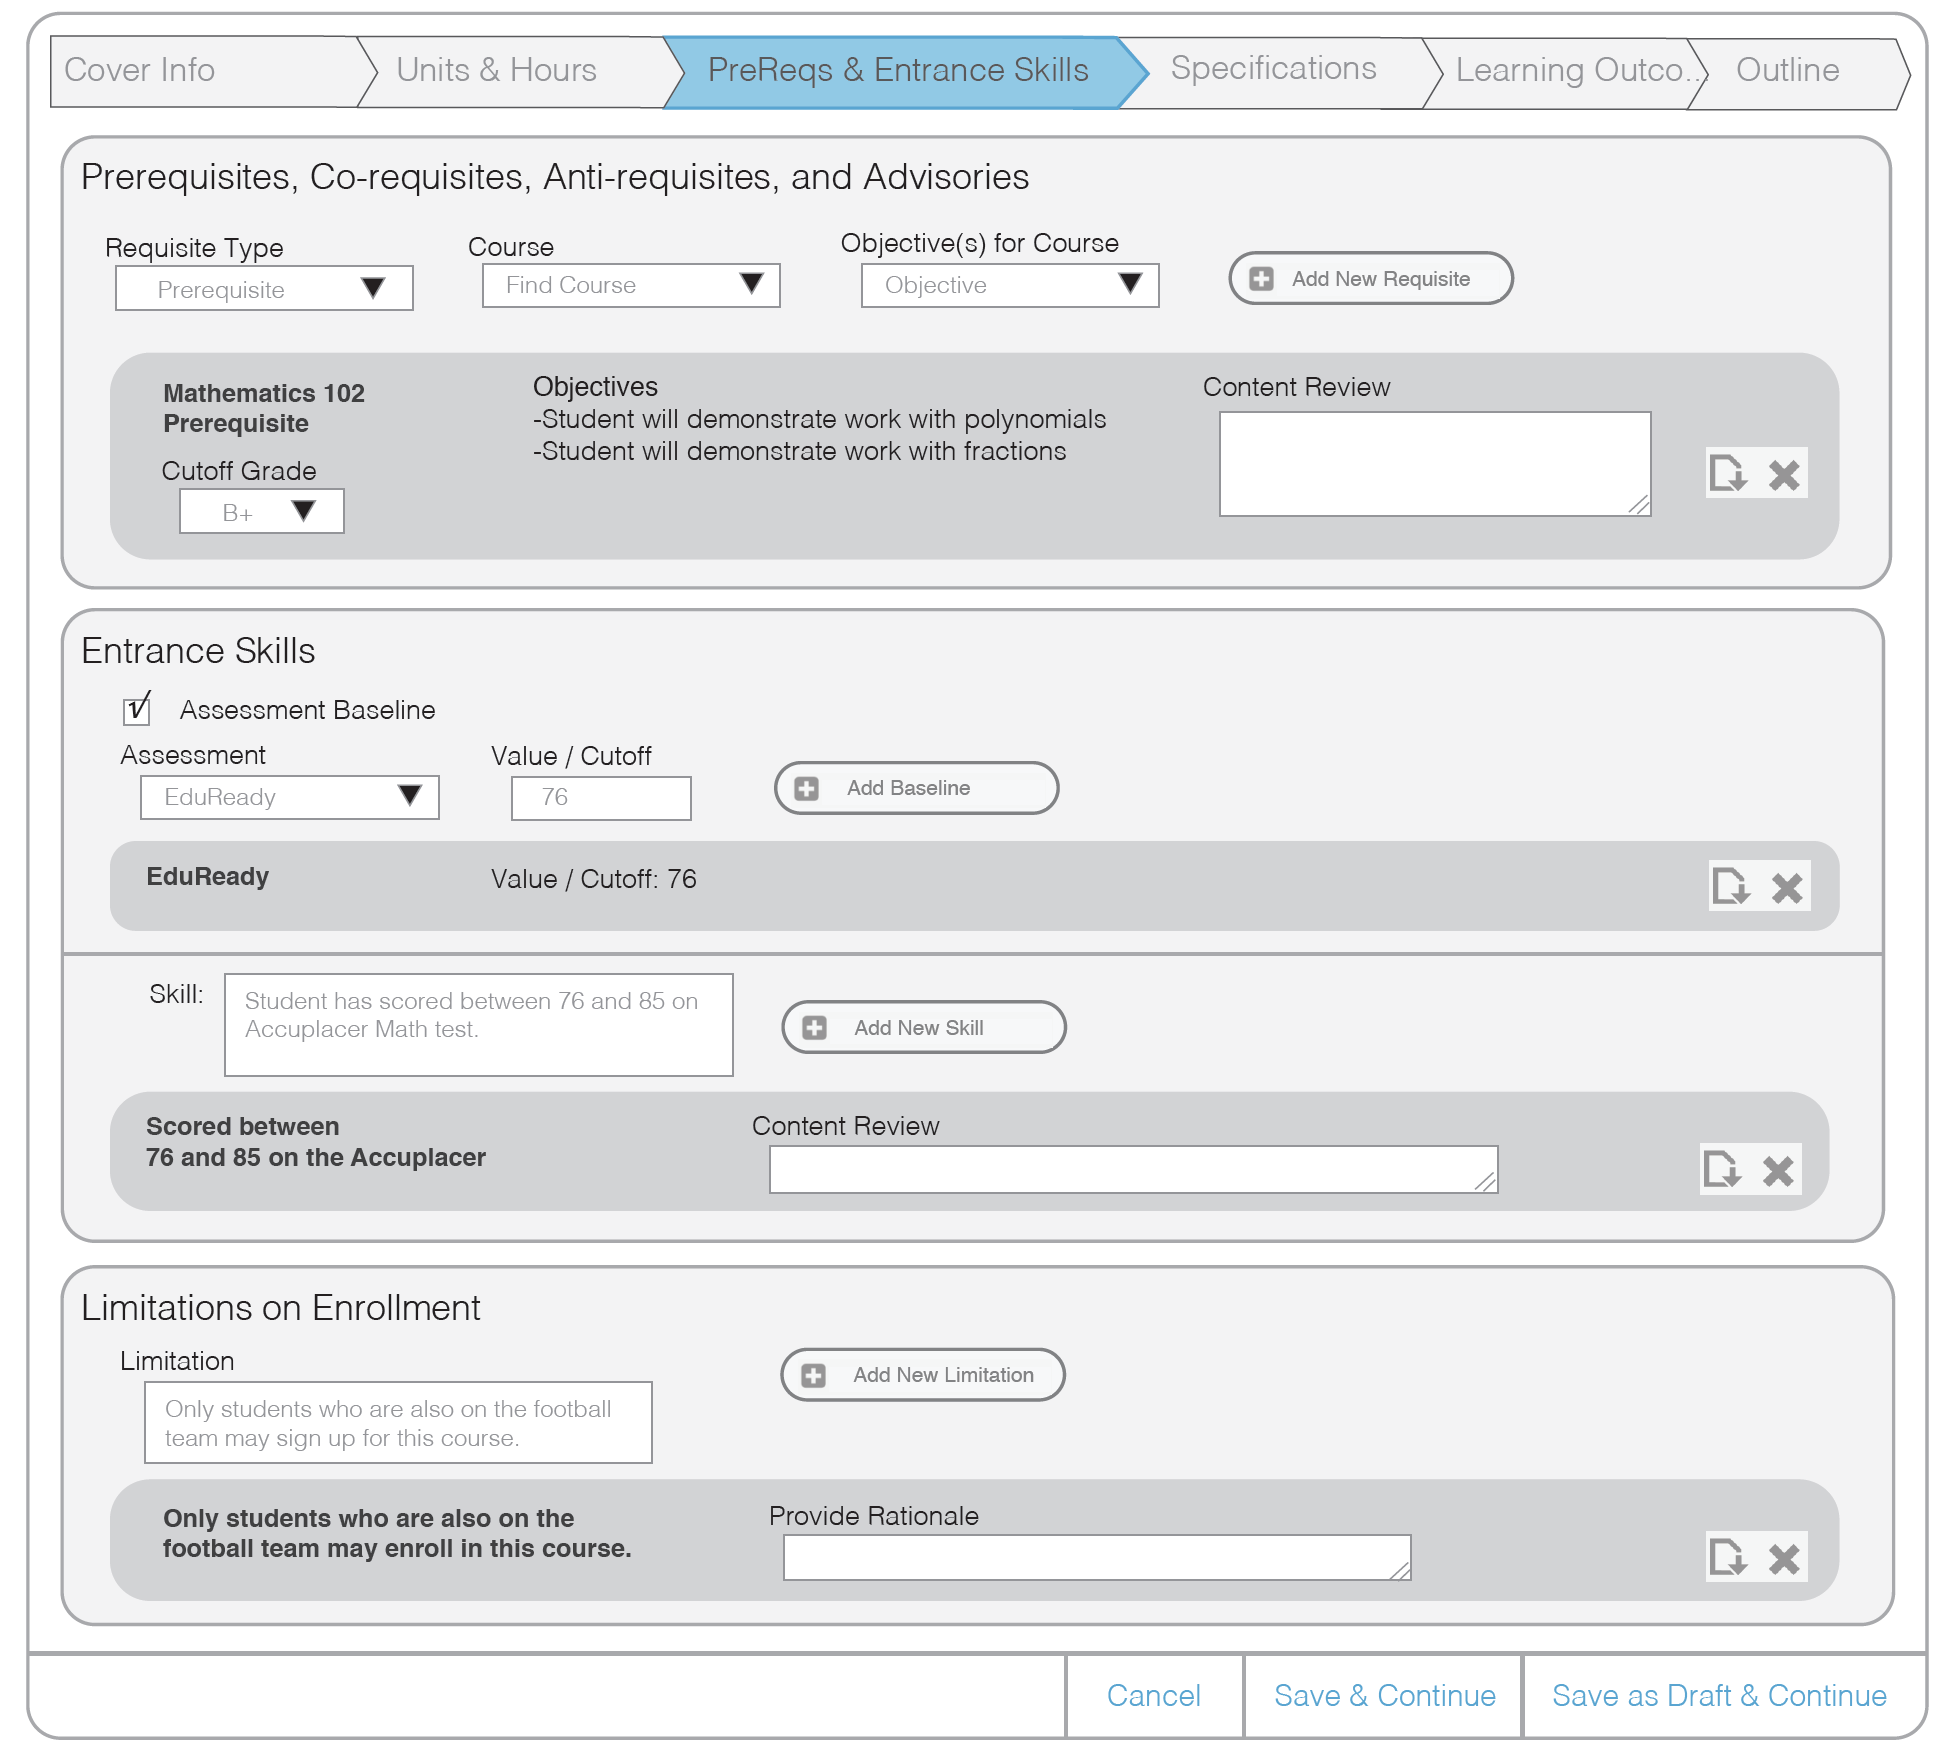
\includegraphics[scale=0.3]{Capitulos/DesarrollodelaAplicacion/Imagenes/course_req}
\caption{Mockup de la pantalla de requisitos de curso.}
  \label{course_req}
\end{figure}

\subsection{Revisar y aprobar curso}
La historia de usuario tiene como criterios de aceptación los siguientes puntos:
\begin{itemize}
	\item Las páginas para revisar los flujos de trabajos tienen una región de retroalimentación o feedback debajo de cada paso, con la opción de ocultar y mostrar para que el usuario que está revisando el flujo de trabajo en desarrollo pueda dejar comentarios al encargado del formulario del curso.
	\item La interfaz tiene elementos de estado que indican que cierta parte es nueva, aprobada, y rechazada.
	\item Los pasos tienen regiones que permiten aceptar o rechazar los campos propuestos por los desarrolladores del curso. Por lo tanto, deben tener elementos de interfaz que indiquen al usuario que puede aprobar o rechazar cada parte.
\end{itemize}
Además de los criterios de aceptación, había que volver a actualizar el buzón de entrada para que acepten los cambios que tiene la historia de usuario. Debido a que más de una persona puede revisar el flujo de trabajo y podría trancar el proceso si es que no se le notifica debidamente que hay nuevos cambios que revisar.

Algunas de las tareas descompuestas de la historia de usuario son las siguientes:
\begin{itemize}
	\item Actualizar el visualizador de flujo de trabajo para que pueda soportar la nueva característica de aprobación o rechazo de cada parte.
	\item Actualizar el buzón de entrada de Cursos.
	\item Pruebas de funcionamiento.
\end{itemize}

La historia se ha terminado en una iteración con 68 horas cargadas de desarrollo

\subsection{Competencias de curso}
Esta historia tiene como propósito de crear o versionar competencias para el curso a ser creado o versionado. 

La organización ha proporcionado mockups (figura \ref{course_learning_outcomes}) para el paso a desarrollarse y era un criterio de aceptación de parte del ticket que siga el mismo formato.

La historia de usuario tiene como descripción: \enquote{\textit{Como encargado del formulario de curso, me gustaría ser capaz de articular las competencias de mi nuevo curso, para de esa manera de tener que estar añadiendo una a una después de completar el proceso de creación de cursos con el flujo}}.

Como criterio de aceptación de la historia fue la de agregar el flujo de trabajo de competencias en el flujo de trabajo de cursos. Algunas de las tareas de la historia fueron:
\begin{itemize}
	\item Modificar la base de datos para que soporte el nuevo modelo de datos de las competencias dentro de flujo de trabajo de curso.
	\item Modificar o agregar clases de las entidades que van a ser usadas durante la historia.
	\item Actualizar la plantilla de flujo de trabajo para que soporte el nuevo paso para la creación o versionamiento de competencias.
	\item Actualizar el visualizador de flujo de trabajo para que soporte el nuevo paso de competencias.
	\item Actualizar los servicios de guardado y de versionamiento de cursos y competencias.
	\item Pruebas de nuevas funcionalidades.
\end{itemize}

La historia ha sido terminada en dos iteraciones con un total de 76 horas cargadas en el sistema.

\begin{figure}[H]
\centering
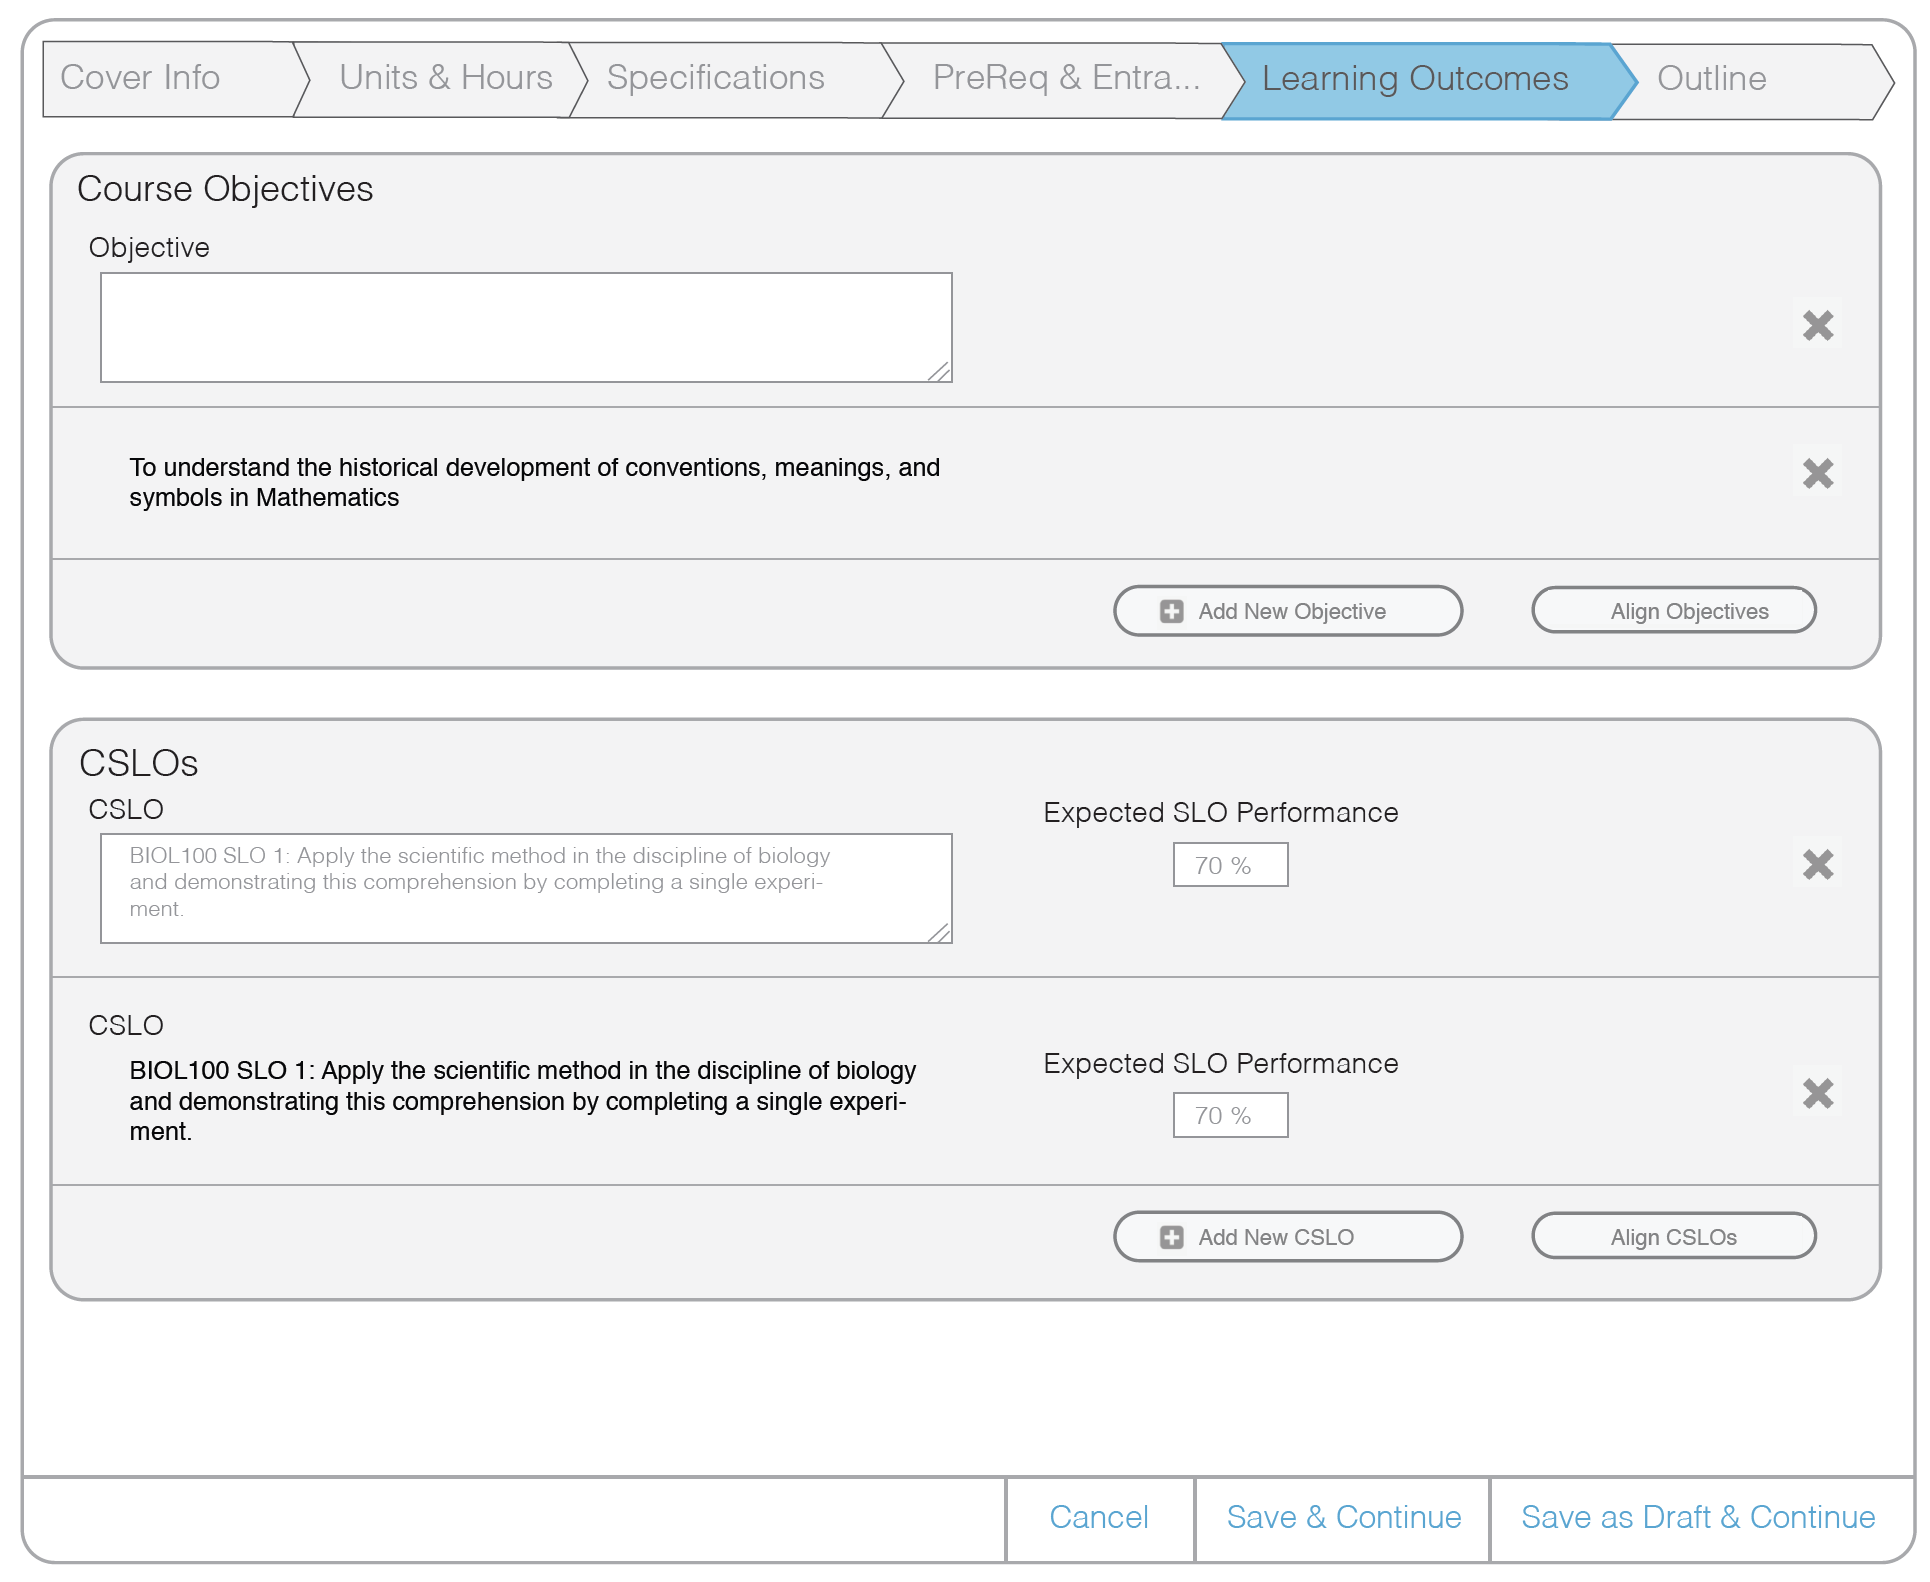
\includegraphics[scale=0.3]{Capitulos/DesarrollodelaAplicacion/Imagenes/course_learning_outcomes}
\caption{Mockup de la pantalla de competencias de curso.}
  \label{course_learning_outcomes}
\end{figure}

\subsection{Esquema de curso}
Esta historia tiene como propósito de diseñar la pantalla para un nuevo paso para el flujo de trabajo. 

La organización ha proporcionado mockups (figura \ref{course_outline}) para el paso a desarrollarse y era un criterio de aceptación de parte del ticket que siga el mismo formato.

La historia de usuario tiene como descripción: \enquote{\textit{Como encargado del formulario de curso, me gustaría ser capaz de agregar el esquema de un curso, para de esta manera dar un resumen de curso para el que esté revisando mi flujo y para que los estudiantes puedan tener una idea de se trata una vez que se curse}}.

Como criterio de aceptación de la historia fue la de agregar el flujo de trabajo de competencias en el flujo de trabajo de cursos. Algunas de las tareas de la historia fueron:
\begin{itemize}
	\item Modificar la base de datos donde se tendría que almacenar los nuevos campos de esquema ya sea para el curso y para el flujo que se desarrolla.
	\item Modificar o agregar clases de las entidades que van a ser usadas durante la historia.
	\item Actualizar la plantilla de flujo de trabajo para que soporte el nuevo paso de esquema de cursos.
	\item Actualizar el visualizador de flujo de trabajo para que soporte el nuevo paso de competencias.
	\item Actualizar los servicios de guardado y de revisión para que soporte nuevo paso.
\end{itemize}

La historia ha sido terminada en dos iteraciones con un total de 48 horas cargadas en el sistema.

\begin{figure}[H]
\centering
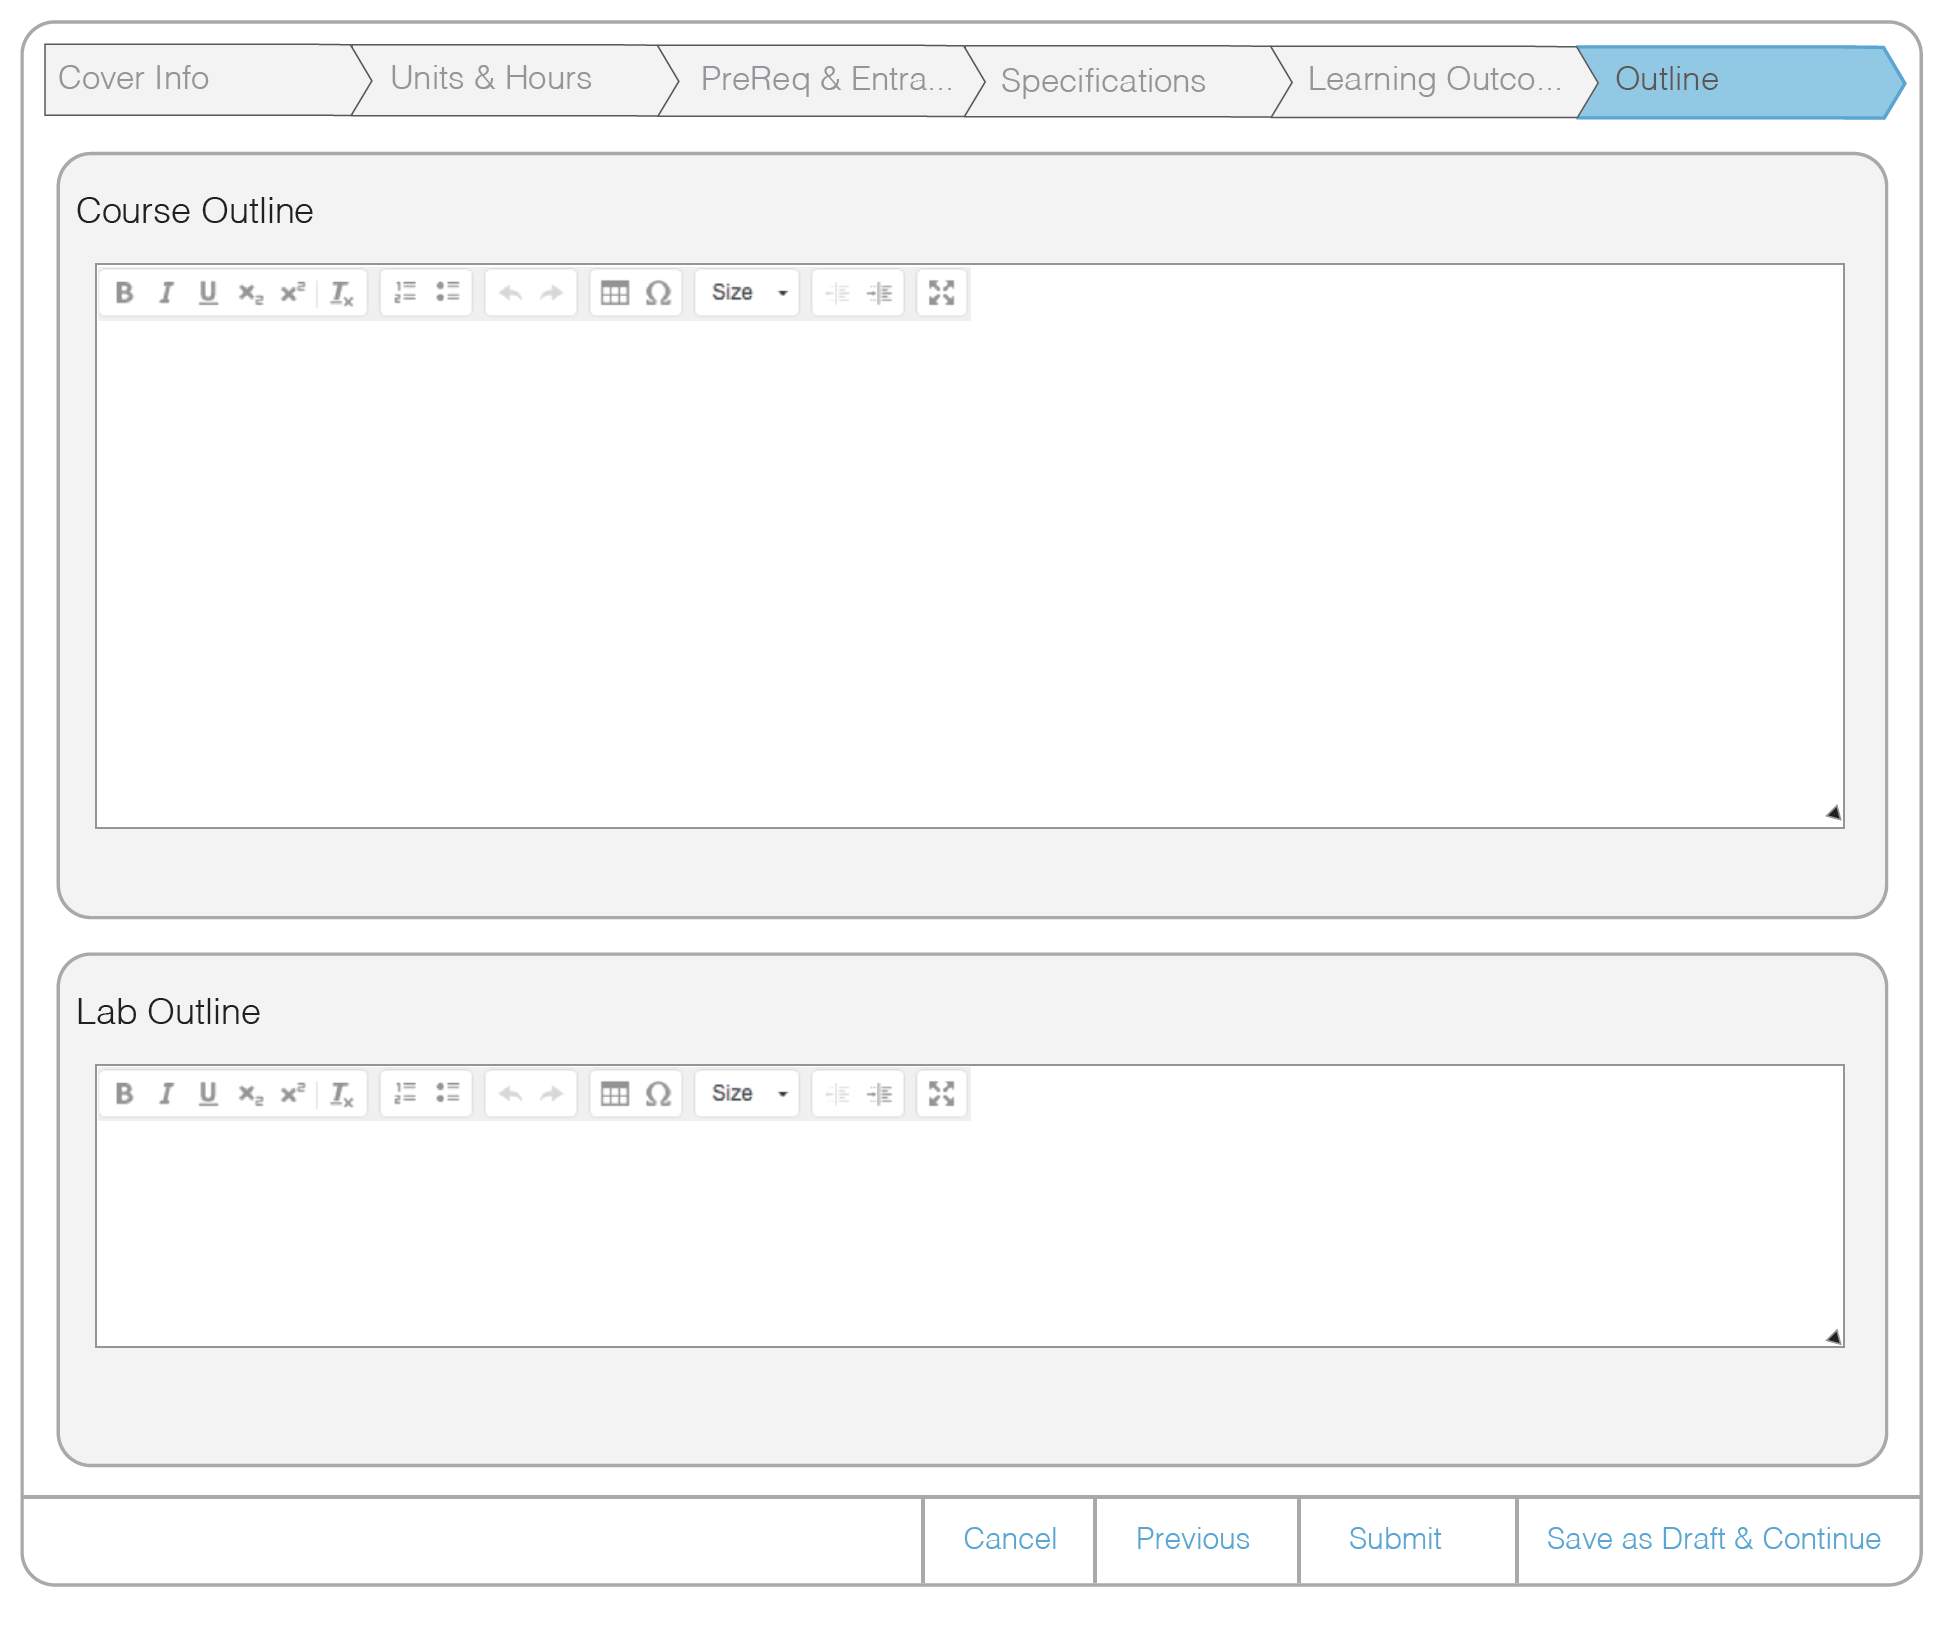
\includegraphics[scale=0.3]{Capitulos/DesarrollodelaAplicacion/Imagenes/course_outline}
\caption{Mockup de la pantalla de esquema de curso.}
  \label{course_outline}
\end{figure}

\subsection{Códigos de clasificación de curso}
Esta historia tiene como propósito la de asignar códigos de clasificación a los cursos.

Para entrar en contexto, habría que definir primero que es TOP\footnote{de sus siglas en inglés, Taxonomy Of Programs, que significa en español taxonomía de programas.}.

TOP es un sistema numérico de códigos usados a nivel de Estado para recolectar y reportar información en cursos y programas, en diferentes instituciones educativas \citep{brice_w_harris_program_2013} por todo el Estado. 

Ha sido diseñado para agregar información acerca de los programas. Sin embargo, un código TOP debe ser asignado a cada curso del sistema. 

Aunque no contiene tantas opciones específicas como lo haría un sistema diseñado para cursos, a cada curso se le debe dar el código que se aproxima a describir el contenido del curso.

Algunos usos a los códigos:
\begin{itemize}
	\item En el inventario de programas aprobados y rechazados, para tener información que tipos de cursos y programas son ofrecidas por el estado.
	\item En bases de datos de administración de información, para recolectar y reportar información en logros estudiantiles (licenciaturas y certificados) en ciertos programas.
	\item En contabilidad vocacional estudiantil, para reportes de compleción de programas y cursos de ciertos programas vocacionales.
\end{itemize}

La historia de usuario tiene como descripción: \enquote{\textit{Como miembro del comité curricular, me gustaría ser capaz de asignar a mis cursos de códigos de clasificación como parte de la aprobación de mis flujo de trabajos para asegurar que estén correctos, como esto es motivo de rechazo en la oficina del canciller del Estado}}.

Algunas de las tareas fueron las siguientes:
\begin{itemize}
	\item Diseño del nuevo modelo, donde se debían generar tablas para cada nueva entidad del modelo de datos ajustado para las taxonomías de programas. Además, cargar todos los datos de códigos de cursos existentes para el estado de California.
	\item Creación de clases Java.
	\item Diseño e implementación páginas CRUD para disciplina, sub-disciplina, y campo.
	\item Diseño e implementación de la nueva página de asignación de códigos de clasificación para los cursos en proceso de diseño.
	\item Hacer servicios para cada una de las nuevas páginas.
	\item Pruebas de funcionalidad.
\end{itemize}

La historia de usuario ha sido terminada en una iteración con 80 horas cargadas en el sistema.
\section{Flujo de trabajo para el versionamiento de programas de estudio}
\begin{table}[H]
\centering
\resizebox{\columnwidth}{!}{%
\begin{tabular}{@{}lllll@{}}
\toprule
Historias de usuario               & HE  & HC  & PH & Sprints \\ \midrule
Información básica del programa    & 54  & 56  & 8  & 1       \\
Competencias de carrera o programa & 48  & 68  & 5  & 1       \\
Bloques de curso                   & 58  & 60  & 5  & 1       \\
Visualizar cambios en los campos   & 180 & 210 & 13 & 4       \\ \bottomrule
\end{tabular}
}
\caption{Historias de usuario para flujo de trabajo para el versionamiento de programas de estudio}
\label{epic:8}
\end{table}

\subsection{Información básica del programa}
La historia de usuario tiene como descripción lo siguiente \enquote{\textit{Como coordinador del departamento o encargado del AMS, me gustaría ser capaz de agregar o revisar programas en el módulo de gestión curricular, para que de esta forma pueda manejar mejor mis registros de la institución en el sistema}}. Y los criterios de aceptación consistían en el desarrollo de la pantalla que se puede apreciar en la figura \ref{program_cover_info}.

Algunas de las tareas identificadas en la planificación de las iteraciones eran los siguientes:
\begin{itemize}
	\item Adaptar la base de datos para soportar los nuevos campos a ser guardados por el flujo de trabajo.
	\item Luego de hacer los cambios en la base de datos, actualizar o agregar nuevas clases de Java para su posterior uso.
	\item Desarrollar la página de información básica del programa.
	\item Actualizar la plantilla de flujos de trabajo institucional para que soporte la creación y revisión de programas.
	\item Diseñar servicios para guardar los registros de la nueva página.
	\item Diseñar servicios de aprobación de flujo de trabajo de programas.
\end{itemize}

La historia fue finalizada en una iteración con una cantidad de 56 horas cargadas en el sistema.

\begin{figure}[H]
\centering
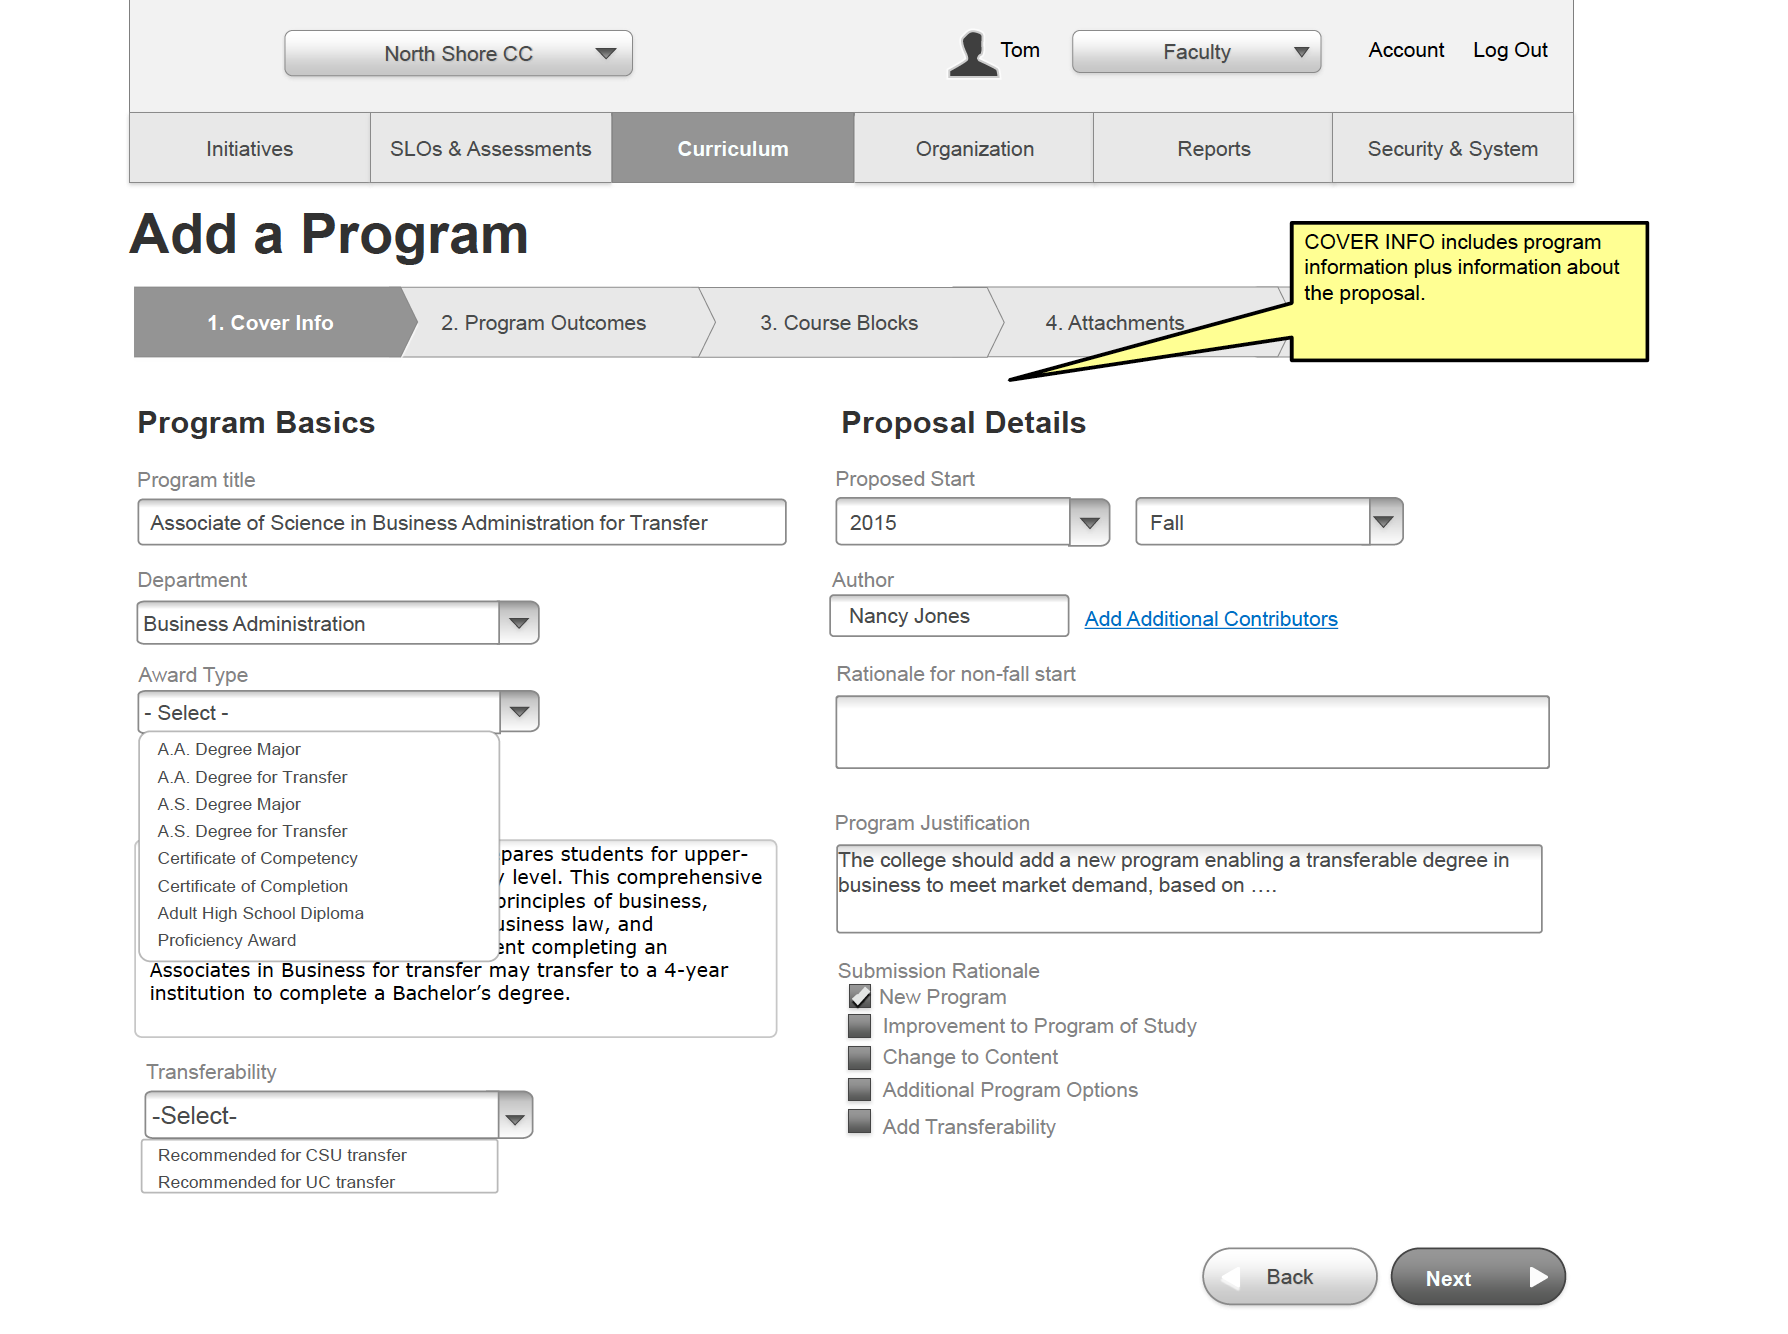
\includegraphics[width=125mm,scale=1]{Capitulos/DesarrollodelaAplicacion/Imagenes/program_cover_info}
\caption{Mockup de la pantalla de información básica del programa.}
  \label{program_cover_info}
\end{figure}

\subsection{Competencias de carrera o programa}
La historia de usuario tiene como descripción lo siguiente \enquote{\textit{Como coordinador, me gustaría ser capaz de administrar las competencias asociadas a mi programas durante el flujo de creación y revisión del mismo, para que pueda hacer una revisión comprensiva de los programas que tiene el AMS}}. Y los criterios de aceptación consistían en el desarrollo de la pantalla que se puede apreciar en la figura \ref{program_learning_outcomes}.

Algunas de las tareas identificadas en la planificación de las iteraciones eran los siguientes:
\begin{itemize}
	\item Adaptar la base de datos para soportar los nuevos campos a ser guardados por el flujo de trabajo.
	\item Luego de hacer los cambios en la base de datos, actualizar o agregar nuevas clases de Java para su posterior uso.
	\item Desarrollar la página de información básica del programa.
	\item Actualizar los servicios de guardado de campos para el flujo de trabajo.
	\item Actualizar los servicios de aprobación de flujo de trabajo de programas.
\end{itemize}

La historia fue finalizada en una iteración con una cantidad de 68 horas cargadas en el sistema.

\begin{figure}[H]
\centering
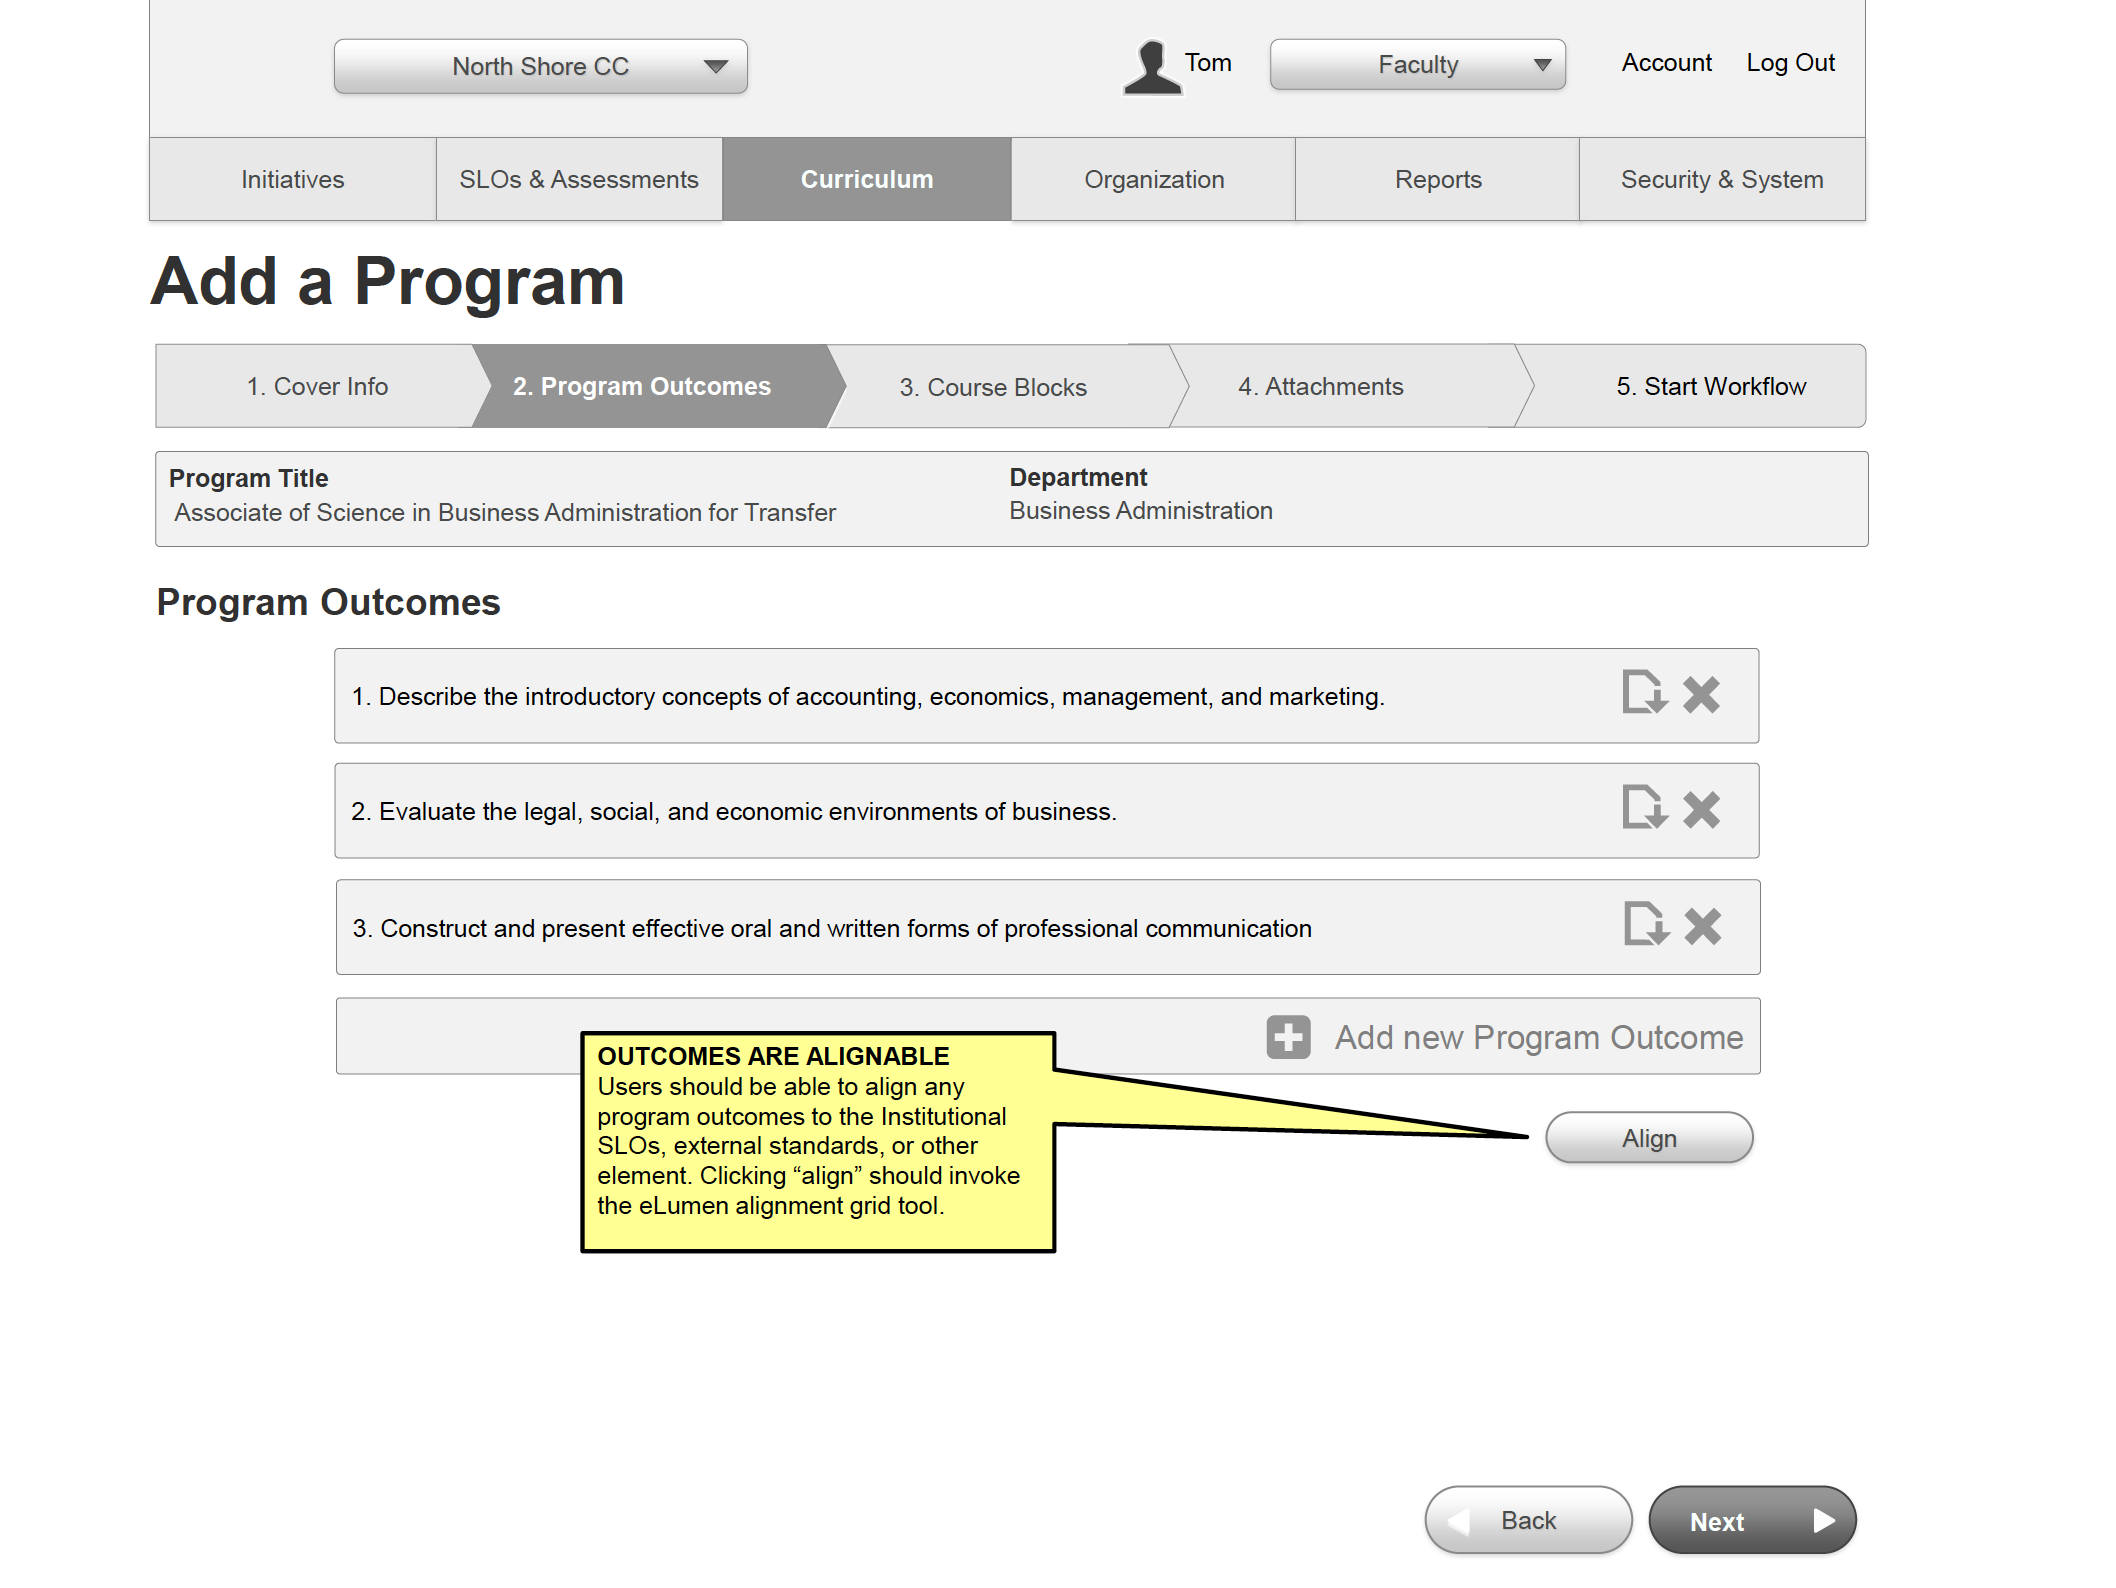
\includegraphics[width=125mm,scale=1]{Capitulos/DesarrollodelaAplicacion/Imagenes/program_learning_outcomes}
\caption{Mockup de la pantalla de competencias del programa.}
  \label{program_learning_outcomes}
\end{figure}

\subsection{Bloques de cursos}
La historia de usuario tiene como descripción lo siguiente \enquote{\textit{Como coordinador de departamento, me gustaría ser capaz de diseñar bloques de cursos para mis programas, para que de esta manera pueda diseñar la malla para mis programas de estudio}}. Y los criterios de aceptación consistían en el desarrollo de la pantalla que se puede apreciar en la figura \ref{program_course_blocks}.

Algunas de las tareas identificadas en la planificación de las iteraciones eran los siguientes:
\begin{itemize}
	\item Diseño e implementación del modelo de datos.
	\item Diseño e implementación de clases Java.
	\item Desarrollar la página de paso para creación de bloques de cursos en los diferentes flujos de trabajo.
	\item Desarrollar servicios de guardado y aprobación de la funcionalidad.
	\item Actualizar la plantilla de flujos de trabajo.
\end{itemize}

La historia fue finalizada en una iteración con una cantidad de 60 horas cargadas en el sistema.

\begin{figure}[H]
\centering
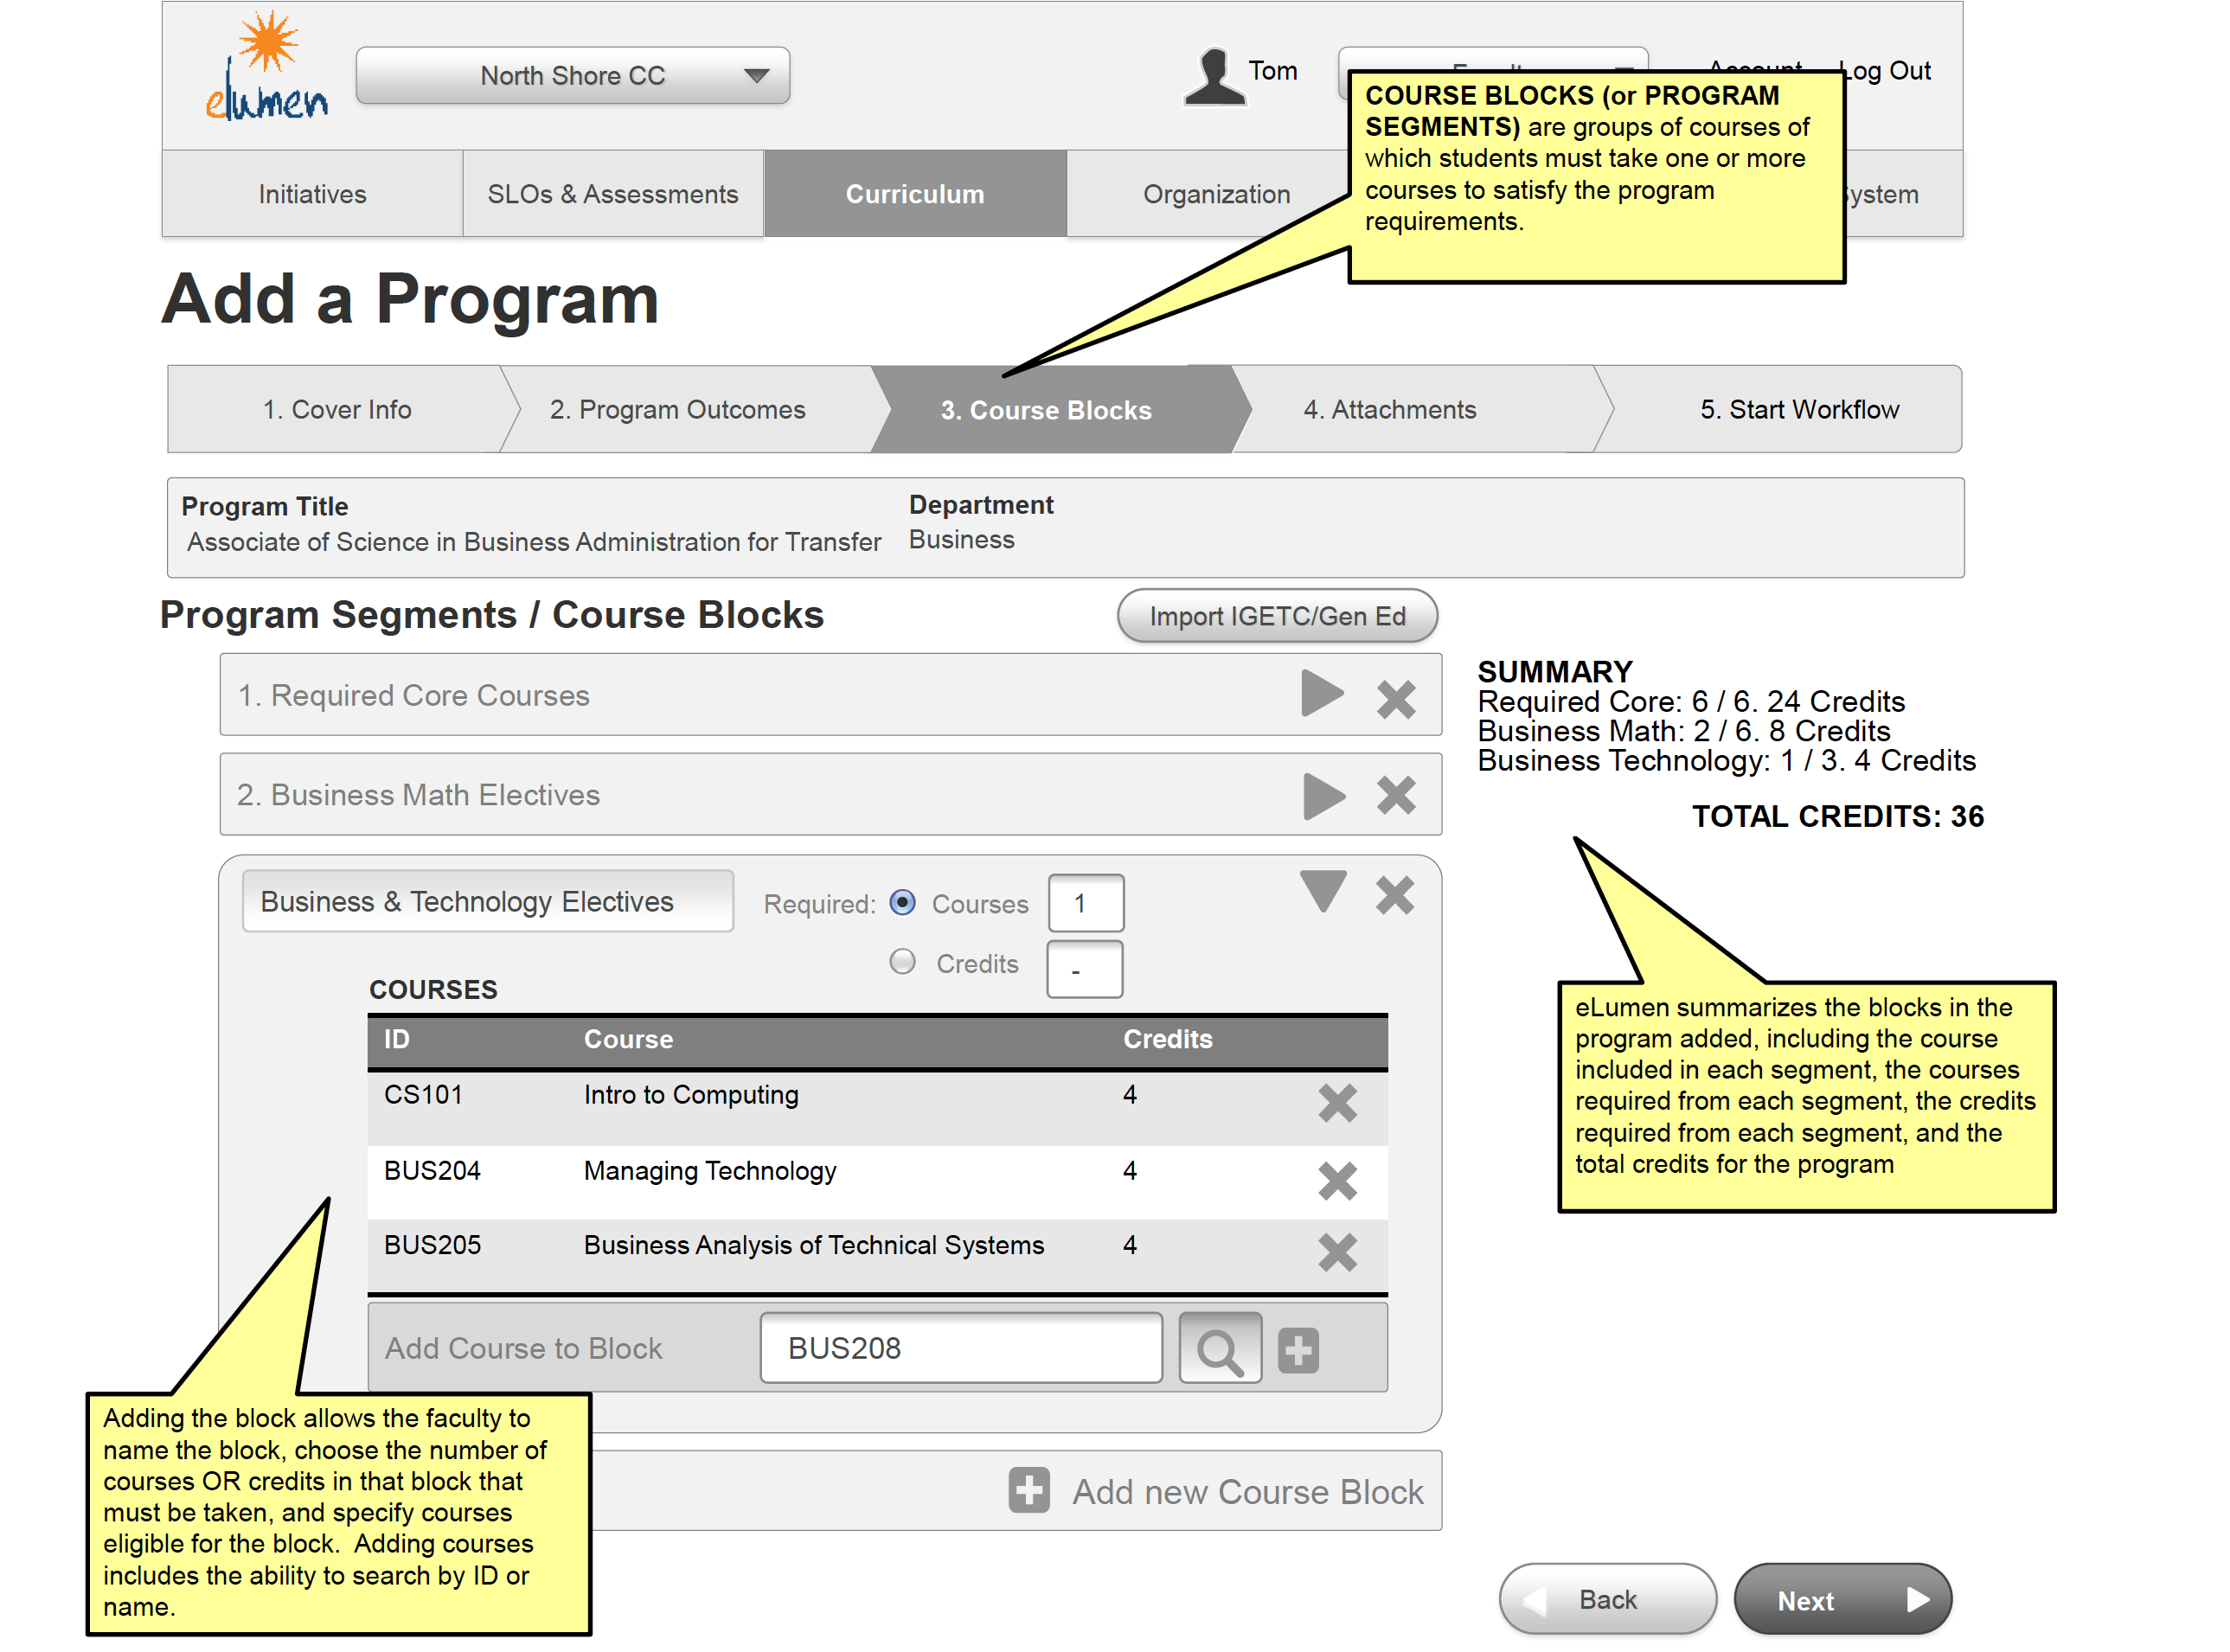
\includegraphics[width=125mm,scale=1]{Capitulos/DesarrollodelaAplicacion/Imagenes/program_course_blocks}
\caption{Mockup de la pantalla de bloques de cursos de programa.}
  \label{program_course_blocks}
\end{figure}

\subsection{Visualizar cambios en los campos}
La historia de usuario tiene como descripción lo siguiente \enquote{\textit{Como coordinador de departamento, me gustaría ser capaz de diseñar bloques de cursos para mis programas, para que de esta manera pueda diseñar la malla para mis programas de estudio}}. Y los criterios de aceptación consistían en el desarrollo de la pantalla que se puede apreciar en la figura \ref{visualize_changes}.

Como criterios de aceptación se encuentran los siguientes:
\begin{itemize}
	\item Los campos borrados se deben marcar en rojo.
	\item Los nuevos campos se deben marcar en verde.
	\item Se debe visualizar el estado anterior y el nuevo con una forma de identificar con el usuario que hizo la modificación.
	\item Limitado para los cambios del programa.
	\item Diseño de interfaz aprobada por el equipo de validación.
	\item Las diferencias limitadas a dos versiones.
\end{itemize}

Algunas de las tareas identificadas en la planificación de las iteraciones eran los siguientes:
\begin{itemize}
	\item Diseño e implementación del modelo de datos.
	\item Diseño e implementación de clases Java.
	\item Desarrollar la página de paso para creación de bloques de cursos en los diferentes flujos de trabajo.
	\item Desarrollar servicios de guardado y aprobación de la funcionalidad.
	\item Actualizar la plantilla de flujos de trabajo.
\end{itemize}

La historia fue finalizada en una iteración con una cantidad de 60 horas cargadas en el sistema.

\begin{figure}[H]
\centering
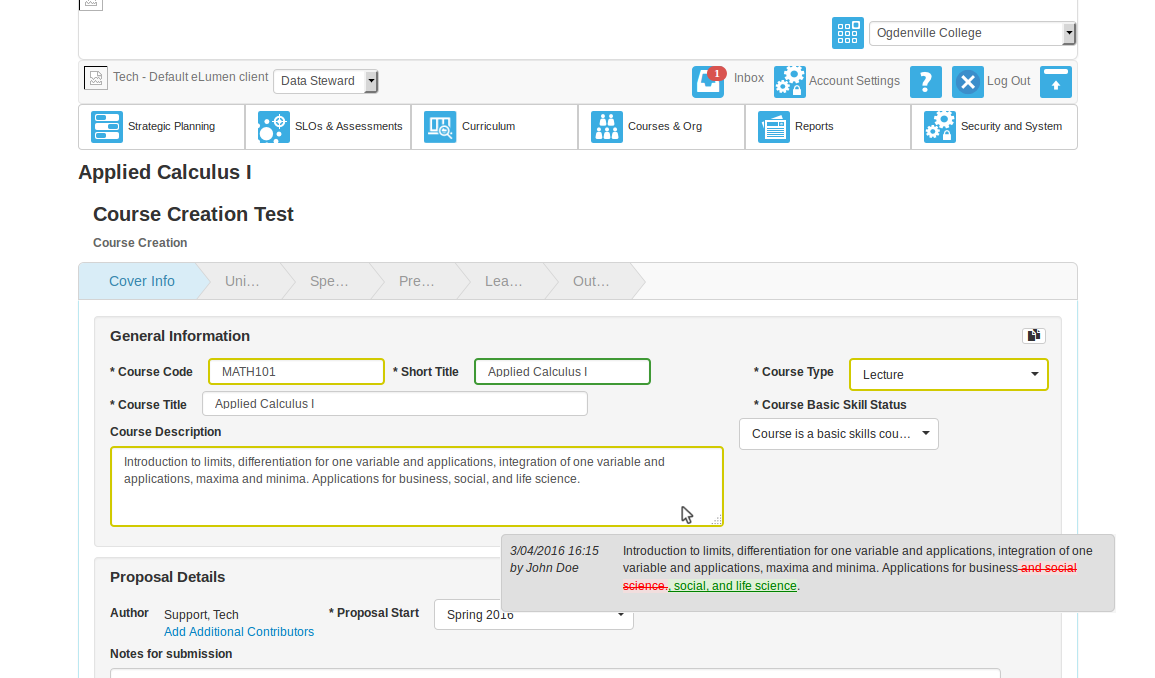
\includegraphics[width=125mm,scale=1]{Capitulos/DesarrollodelaAplicacion/Imagenes/visualize_changes}
\caption{Mockup de la pantalla de la funcionalidad de visualización de cambios.}
  \label{visualize_changes}
\end{figure}

\section{Soporte de etapas en los flujos de trabajo}
\begin{table}[H]
\centering
\resizebox{\columnwidth}{!}{%
\begin{tabular}{@{}lllll@{}}
\toprule
Historias de usuario                                             & HE  & HC  & PH & Sprints \\ \midrule
Roles de creación y edición para las partes de flujos de trabajo & 102 & 112 & 13 & 1       \\
Diseño e implementación de etapas                                & 288 & 505 & 21 & 3       \\
Mejora en comportamientos para las etapas por roles              & 84  & 108 & 8  & 2       \\
Composición de etapas y partes                                   & 216 & 391 & 13 & 3       \\
Etapas y partes opcionales en la revisión del flujo              & 64  & 76  & 8  & 1       \\ \bottomrule
\end{tabular}
}
\caption{Historias de usuario para soporte de etapas en los flujos de trabajo}
\label{epic:8}
\end{table}

\subsection{Roles de creación y edición para las partes de flujos de trabajo}
La historia de usuario tiene como descripción lo siguiente \enquote{\textit{Como participante en el proceso curricular, podría no solo revisar nuevos cursos y programas, sino que también realizar pequeñas revisiones como parte del proceso o participe también en el paso de compleción del formulario}}.

Como criterios de aceptación se encuentran los siguientes:
\begin{itemize}
	\item Diseñar el privilegio de creador que permitan a un iniciador de flujo o un diseñador de flujo que designe a ciertos roles para escribir o llenar cada paso.
	\item Diseñar el privilegio de editor que permita editar partes a los que revisan el flujo de trabajo antes de aceptar o rechazar.
	\item Configurar flujos de trabajo para que en cada parte o etapa de un flujo de trabajo puedan ser asignados por roles para la tarea de creador o evaluador, o ambos.
\end{itemize}

Algunas de las tareas identificadas en la planificación de las iteraciones eran los siguientes:
\begin{itemize}
	\item Diseñar e implementar nuevos modelos de datos que permitan soportar el uso de roles para creadores y editores de partes.
	\item Diseñar e implementar servicios de visualización para las diferentes secciones de flujos de trabajo.
	\item Actualizar las plantillas de flujo de trabajo para agregar el soporte de roles de creación y edición.
	\item Actualizar el flujo de trabajo para soportar la compleción de secciones por paso.
	\item Implementar la funcionalidad de edición.
\end{itemize}

La historia fue finalizada en tres iteraciones con una cantidad de 112 horas cargadas en el sistema.


\subsection{Diseño e implementación de Etapas}
La historia de usuario tiene como descripción lo siguiente \enquote{\textit{Como administrador curricular quiero ser capaz de configurar mi plantilla de flujo de trabajo para que pueda dividir en etapas donde se especifiquen que roles pueden completar que funciona en una o múltiples secciones o partes de mi programa o curso}}. Y los criterios de aceptación consistían en el desarrollo de la pantalla que se puede apreciar en la figura \ref{visualize_changes}.

Como criterios de aceptación se encuentran los siguientes:
\begin{itemize}
	\item En un diseño de flujo de trabajo se debe elegir un rol, sección o parte y la acción (completar, revisar, aprobar).
	\item Para la primera etapa solo la acción de completar debe estar disponible.
	\item Las acciones de revisar y aprobar deben estar disponibles si una etapa anterior tiene las mismas secciones o partes con la acción de completar.
	\item Para la primera etapa todas las secciones o partes deben ser completadas en orden secuencial.
	\item Cualquier etapa después de la primera puede tener la opción de mostrar comentarios para la persona que completó los datos antes de transicionar a la siguiente etapa.
\end{itemize}

Algunas de las tareas identificadas en la planificación de las iteraciones eran los siguientes:
\begin{itemize}
	\item Analizar las zonas posibles a ser afectadas por la nueva funcionalidad.
	\item Actualizar la plantilla de flujos de trabajo.
	\item Actualizar el flujo de trabajo de cursos.
	\item Actualizar el flujo de trabajo de programas.
	\item Diseñar e implementar un modelo de datos que soporte la nueva funcionalidad.
	\item Actualizar el buzón de entrada.
	\item Actualizar las notificaciones a colaboradores.
	\item Diseñar e implementar migraciones de datos.
\end{itemize}

La historia fue finalizada en tres iteraciones con una cantidad de 505 horas cargadas en el sistema.

\begin{figure}[H]
\centering
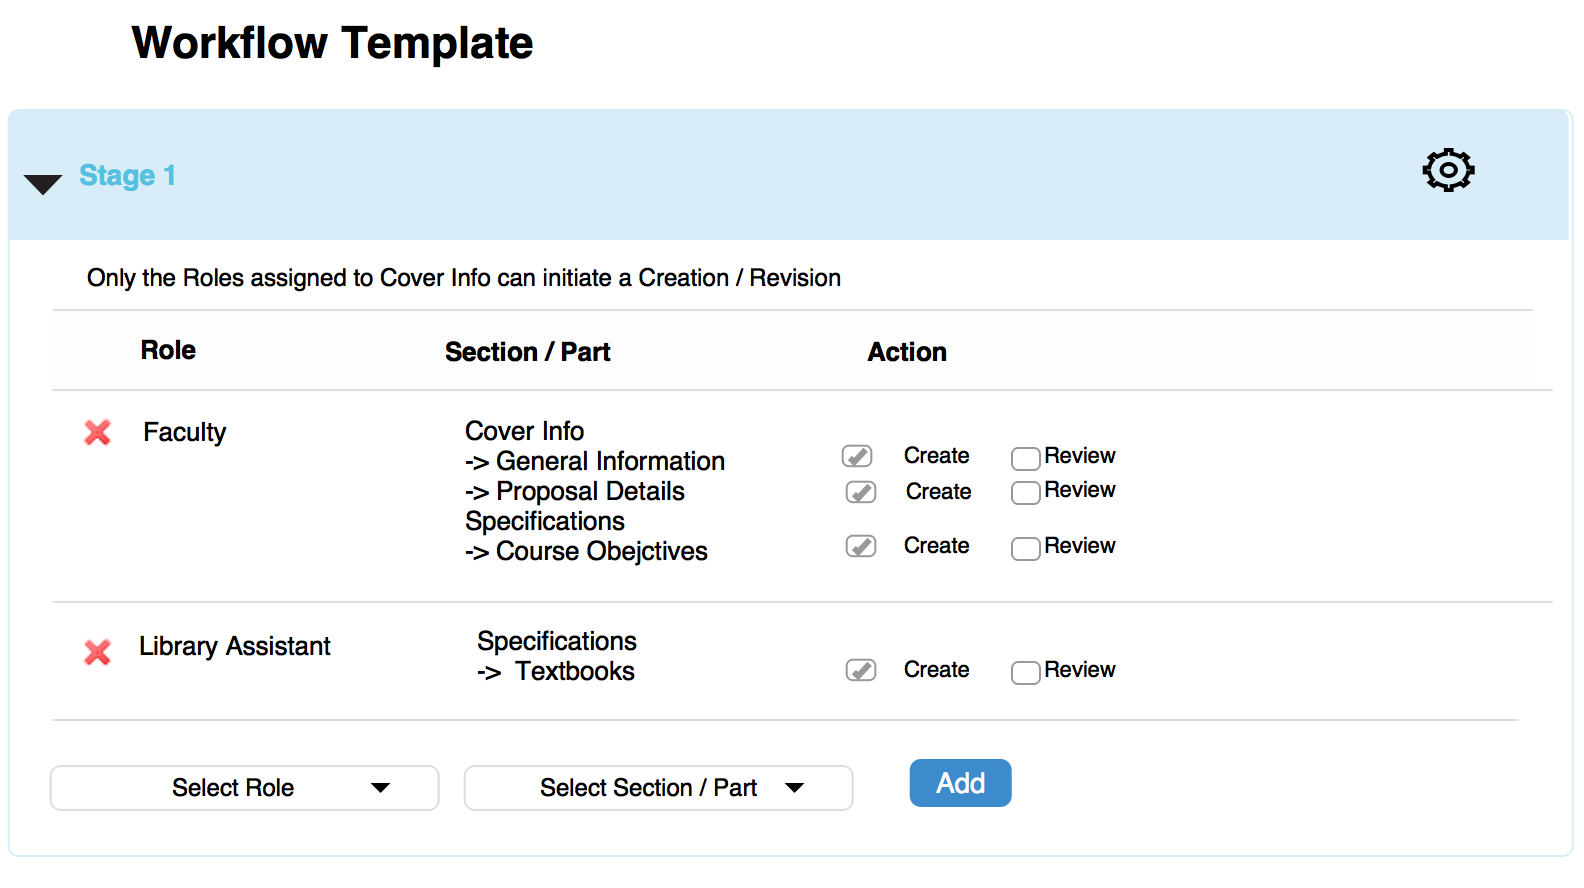
\includegraphics[width=125mm,scale=1]{Capitulos/DesarrollodelaAplicacion/Imagenes/workflow_stage}
\caption{Mockup de la pantalla de plantillas soportando las etapas.}
  \label{workflow_stage}
\end{figure}

\begin{figure}[H]
\centering
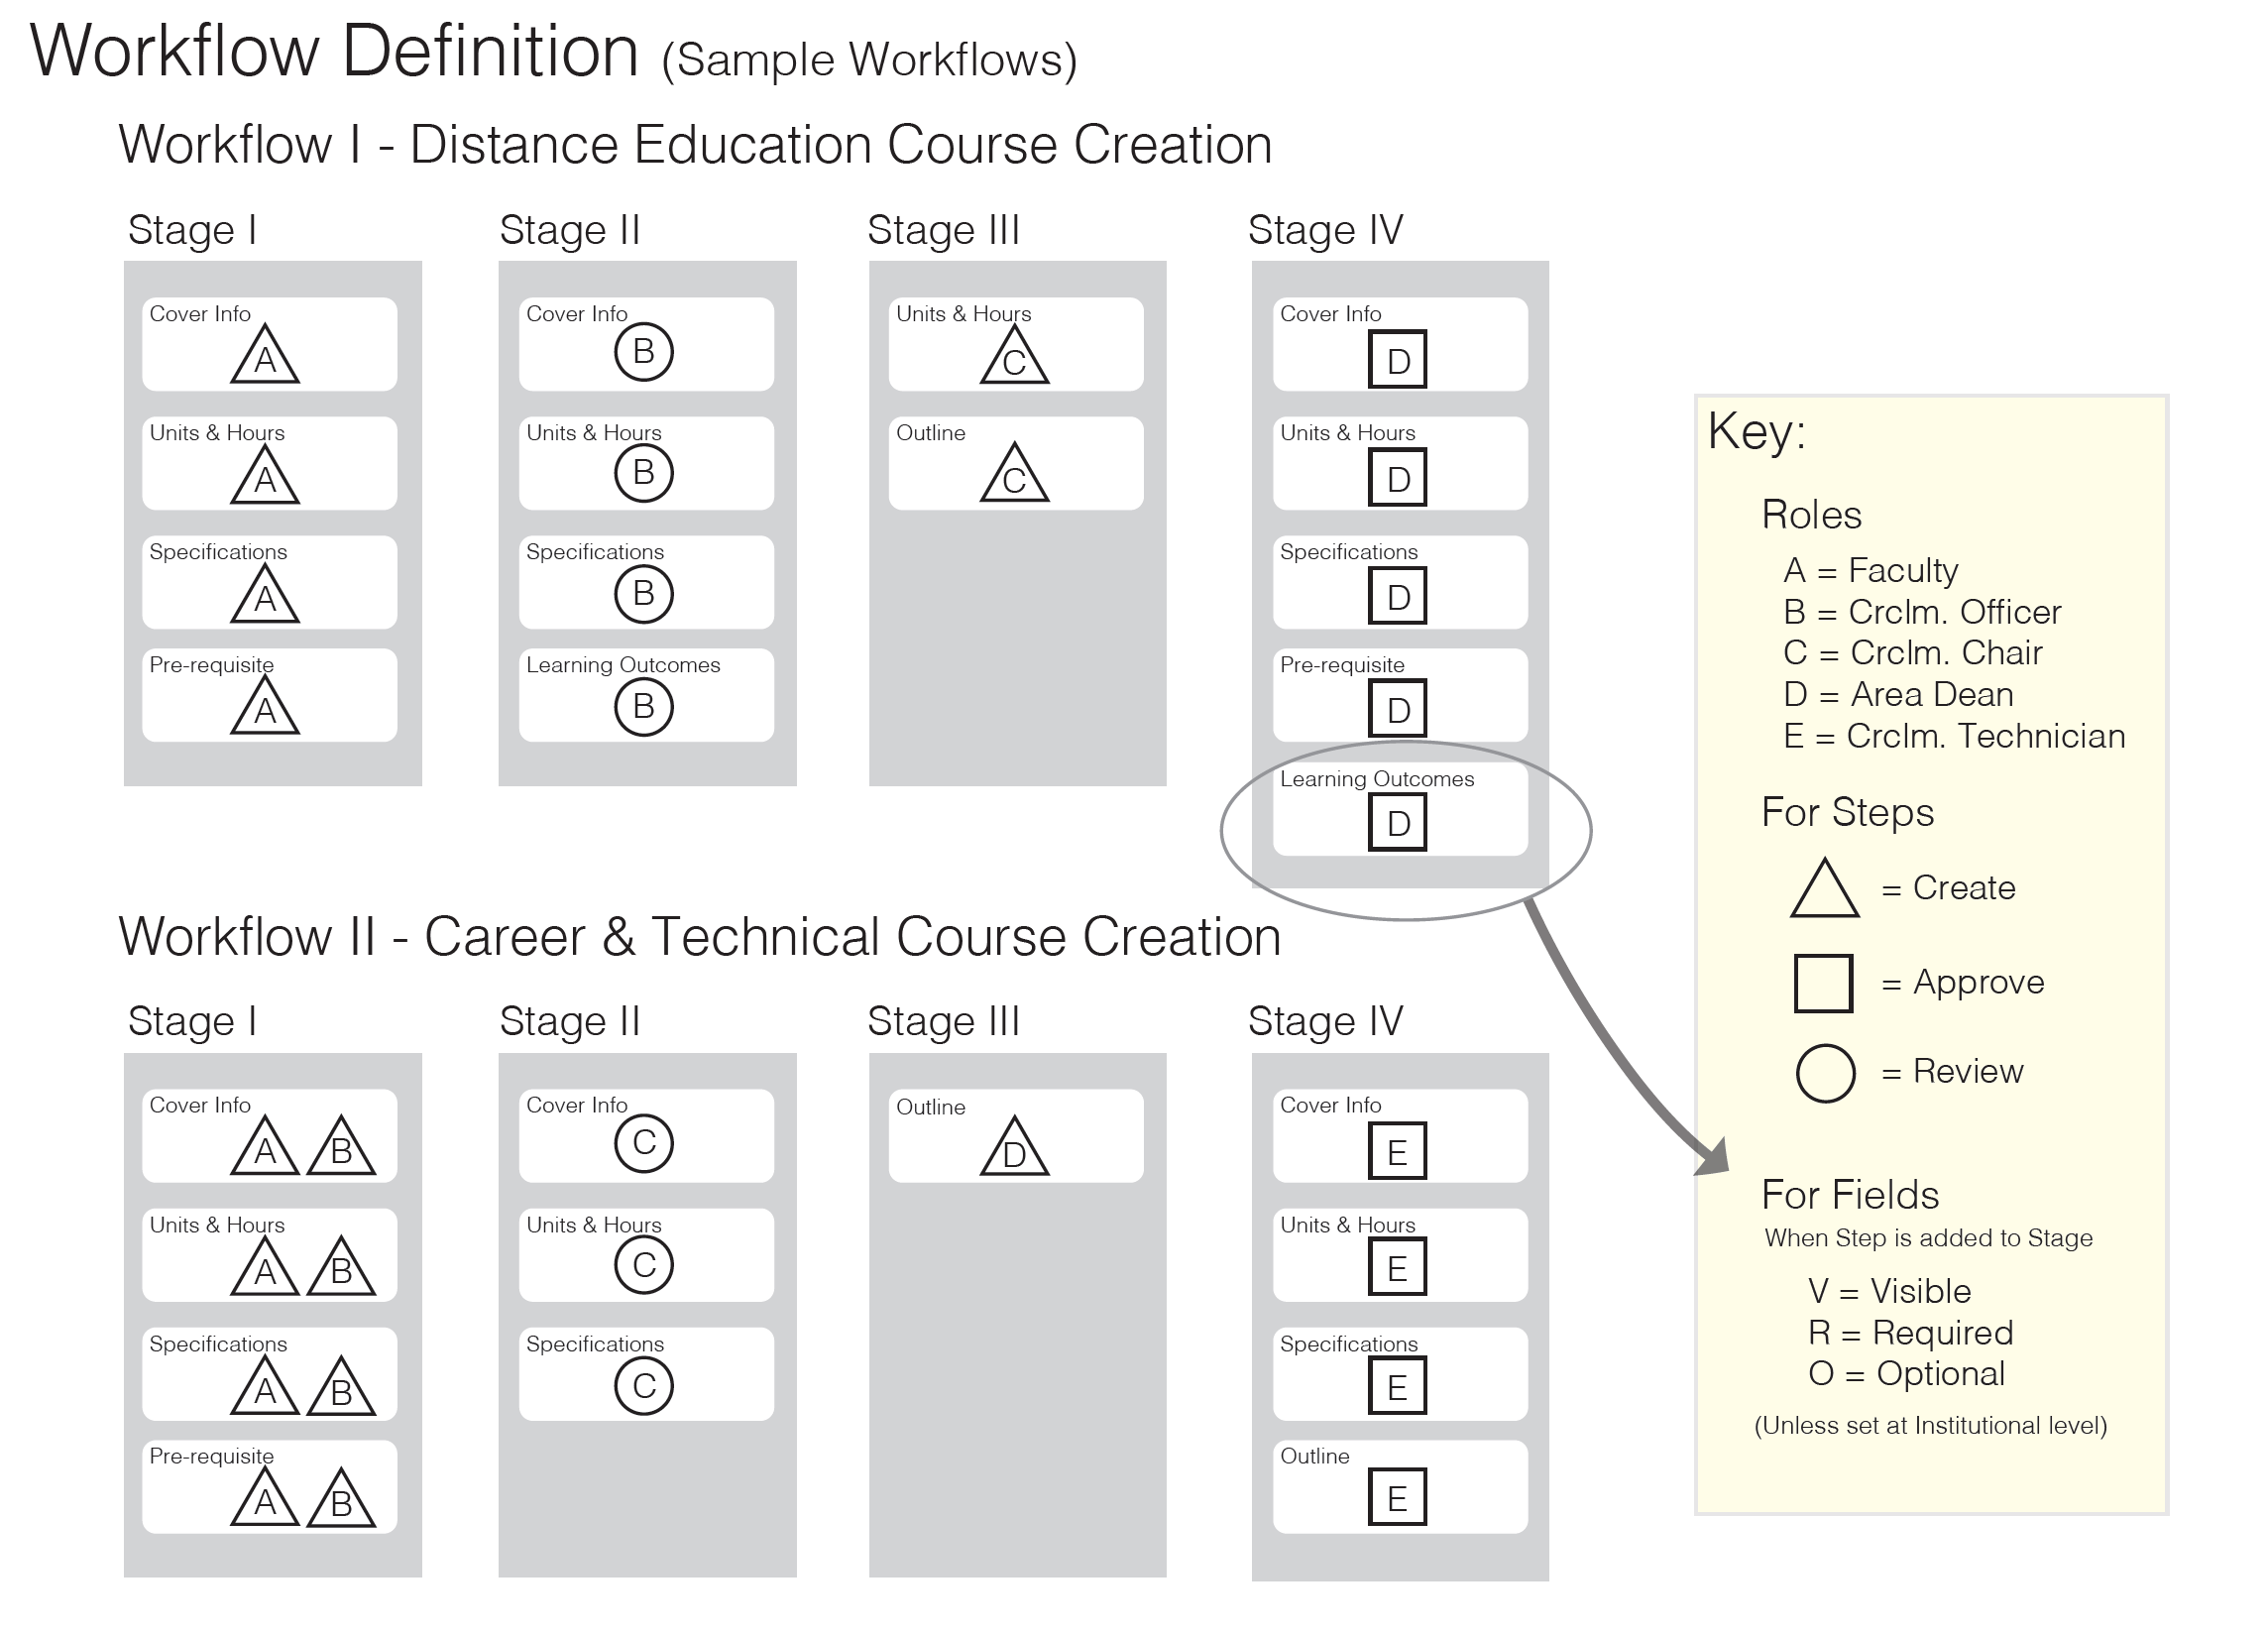
\includegraphics[width=125mm,scale=1]{Capitulos/DesarrollodelaAplicacion/Imagenes/workflow_template_stage}
\caption{Mockup de la pantalla de plantillas con etapas por flujo.}
  \label{workflow_template_stage}
\end{figure}

\subsection{Mejora en comportamientos para las etapas por roles}
La historia de usuario tiene como descripción lo siguiente \enquote{\textit{Como coordinador de educación a distancia, yo solo necesito revisar el esquema del curso para aquellos cursos diseñados para educación a distancia}}.

El criterio de aceptación de la historia consistía en permitir que una etapa que no tiene roles asignados sea opcional.

Algunas de las tareas identificadas en la planificación de las iteraciones eran los siguientes:
\begin{itemize}
	\item Diseñar un plan de pruebas, en estas se identifican las posibles zonas afectadas por la nueva funcionalidad.
	\item Actualizar la pantalla de creación de flujos de trabajo.
	\item Actualizar el mecanismo de transición de etapas.
	\item Mejorar la UI de la vista de etapas de flujos.
\end{itemize}

La historia fue finalizada en tres iteraciones con una cantidad de 108 horas cargadas en el sistema.

\subsection{Composición de etapas y partes}
La historia de usuario tiene como descripción lo siguiente \enquote{\textit{Como presidente curricular, me gustaría ser capaz de componer flujos de trabajo de cursos o programas y etapas (incluyendo actores en cada etapa y sus acciones), para que de esa manera se pueda modelar el proceso curricular en la aplicación}}.

Como criterios de aceptación se encuentran los siguientes:
\begin{itemize}
	\item Cada etapa puede contener una o más partes.
	\item Los actores de cada etapa pueden asignarse actiones a cada parte, o a todas.
	\item Etapas equivalentes no pueden bloquearse entre sí. Por ejemplo, si Suzy y Joe son evaluadores de tres partes, Joe no tiene que esperar que Suzy revise la parte 1 antes de que el pueda evaluar la parte 2, es decir, ambos pueden evaluar sus partes en simultáneo.
\end{itemize}

Algunas de las tareas identificadas en la planificación de las iteraciones eran los siguientes:
\begin{itemize}
	\item Diseño de mockups para su aprobación previa al desarrollo.
	\item Diseño e implementación del modelo de datos que soporte la nueva funcionalidad.
	\item Actualizar las plantillas de flujos de trabajo.
	\item Actualizar los flujos de trabajo de cursos y programas.
	\item Actualizar el sistema de notificaciones.
\end{itemize}

La historia fue finalizada en tres iteraciones con una cantidad de 391 horas cargadas en el sistema.

\subsection{Etapas y partes opcionales en la revisión del flujo}
La historia de usuario tiene como descripción lo siguiente \enquote{\textit{Como administrador curricular quiero ser capaz de configurar mi plantilla de flujo de trabajo para que pueda dividir en etapas donde se especifiquen que roles pueden completar que funciona en una o múltiples secciones o partes de mi programa o curso}}.

Como criterios de aceptación se encuentran los siguientes:
\begin{itemize}
	\item Los roles pueden ser configurados para la acción de creación o revisar, o ambos.
	\item El rol de creación lleva el nombre de creador y para la revisión lleva el nombre de evaluador.
\end{itemize}

Algunas de las tareas identificadas en la planificación de las iteraciones eran los siguientes:
\begin{itemize}
	\item Diseñar un plan de pruebas, en estas se identifican las posibles zonas afectadas por la nueva funcionalidad.
	\item Actualizar la pantalla de creación de flujos de trabajo.
	\item Actualizar el mecanismo de transición de etapas.
\end{itemize}

La historia fue finalizada en tres iteraciones con una cantidad de 76 horas cargadas en el sistema.
\section{Reportes y notificaciones para flujos de trabajo}
\begin{table}[H]
\centering
\caption{Historias de usuario para los reportes y notificaciones de versiones de cursos}
\label{epic:9}
\resizebox{\columnwidth}{!}{%
\begin{tabular}{@{}lllll@{}}
\toprule
Historias de usuario                     			& HE & HC & PH & Sprints \\ \midrule
Notificaciones para las partes del flujo de trabajo & 58 & 60 &  5 &  1 \\
Reporte de esquemas de curso 						& 88 & 91 &  8 &  2 \\ \bottomrule
\end{tabular}
}
\end{table}

\subsection{Notificaciones para las partes del flujo de trabajo}
La historia de usuario tiene como descripción lo siguiente \enquote{\textit{Como especialista curricular, me gustaría que mi equipo de diseño y revisión de flujos de trabajo reciban las notificaciones cuando tengan trabajos pendientes (y alertas cuando este retrasado), para que pueda manejar mejor mis procesos curriculares}}.

Como criterios de aceptación se encuentran los siguientes:
\begin{itemize}
	\item Establecer notificaciones cuando las partes del flujo de trabajo son asignadas a los roles de las personas.
	\item Establecer notificaciones de alerta a asignaciones de partes y etapas. Por ejemplo, 5 días después de su asignación.
	\item Mandar notificaciones por mail.
\end{itemize}

Algunas de las tareas identificadas en la planificación de las iteraciones eran los siguientes:
\begin{itemize}
	\item Diseñar e implementar nuevos modelos de datos que permitan soportar el uso de roles para creadores y editores de partes.
	\item Actualizar el sistema de notificaciones del AMS.
	\item Diseñar e implementar la página de configuración de notificaciones.
\end{itemize}

La historia fue finalizada en tres iteraciones con una cantidad de 60 horas cargadas en el sistema.

\subsection{Reporte de esquemas de curso}
La historia de usuario tiene como descripción lo siguiente \enquote{\textit{Como especialista curricular, me gustaría ser capaz de hacer reportes de registro de esquemas de curso, para que pueda de esta manera ser compartidas por los diferentes colaboradores}}.

Como criterios de aceptación se encuentran los siguientes:
\begin{itemize}
	\item Reporte diseñado por el equipo de diseño curricular.
	\item Incluir competencias es opcional para el reporte.
	\item Incluir alineación de competencias es opcional para el reporte.
	\item Formatos en DOC, PDF o HTML (no Excel).
	\item Se puede ejecutar desde la lista de cursos o de la lista de reportes.
	\item Cuando se corre desde la lista de reportes se pueden elegir uno o más cursos.
\end{itemize}

Algunas de las tareas identificadas en la planificación de las iteraciones eran los siguientes:
\begin{itemize}
	\item Diseñar e implementar el reporte.
	\item Implementar los métodos que acceden a la base de datos.
	\item Diseñar e implementar la página de generación de reportes.
\end{itemize}

La historia fue finalizada en tres iteraciones con una cantidad de 111 horas cargadas en el sistema.
\section{Soporte de versionamiento en el AMS}
\begin{table}[H]
\centering
\caption{Historias de usuario para soporte de versionamiento en el AMS}
\label{epic:10}
\resizebox{\columnwidth}{!}{%
\begin{tabular}{lllll}
\hline
Historias de usuario                                                           & HE & HC & PH & Sprints \\ \hline
Interfaz de alineación de códigos TOP/CIP                                      & 32 & 36 &  3 &  1 \\ 
Renombrar/Reorganizar pestañas para una mejor apariencia del módulo curricular & 32 & 44 &  3 &  1 \\
Lista curricular mejorada para cursos y programas                              &132 &135 &  8 &  2 \\ \hline
\end{tabular}
}
\end{table}

\subsection{Interfaz de alineación de códigos TOP/CIP}
La historia de usuario tiene como descripción lo siguiente \enquote{\textit{Como encargado del sistema de gestión de evaluaciones, me gustaría ser capaz de mantener alineados los codigos TOP a los códigos federales CIP y de esta manera no tener que depender de los administradores para manejar o interpretar estos datos}}.

Como criterios de aceptación se encuentran los siguientes:
\begin{itemize}
	\item Diseñar e implementar una página CRUD para códigos TOP/CIP.
	\item Permitir alinear los códigos.
\end{itemize}

Algunas de las tareas identificadas en la planificación de las iteraciones eran los siguientes:
\begin{itemize}
	\item Diseñar mockups para la nueva página.
	\item Diseñar e implementar el modelo de datos que soporte la funcionalidad.
	\item Desarrollar la página y los métodos de guardado.
\end{itemize}

La historia fue finalizada en una iteración con una cantidad de 36 horas cargadas en el sistema.

\subsection{Reorganización de pestañas para una mejor apariencia del módulo curricular}
La historia de usuario tiene como descripción lo siguiente \enquote{\textit{Como presidente del comité curricular, me gustaría ver las pestañas que están enfocadas a mi trabajo para que pueda navegar y manejar mi tiempo en la aplicación}}.

Como criterios de aceptación se encuentran los siguientes:
\begin{itemize}
	\item Crear pestaña curricular.
	\item Identificar y esconder pestañas no relevantes para el rol.
\end{itemize}

Algunas de las tareas identificadas en la planificación de las iteraciones eran los siguientes:
\begin{itemize}
	\item Diseño de pestañas.
	\item Implementación de pestañas y modificaciones de espacio.
\end{itemize}

La historia fue finalizada en una iteración con una cantidad de 44 horas cargadas en el sistema.


\subsection{Lista curricular mejorada para cursos y programas}
La historia de usuario tiene como descripción lo siguiente \enquote{\textit{Como presidente curricular o miembro del plantel de profesores, me gustaría ser capaz de ordenar/filtrar/visualizar mis cursos y programas, para que de esta manera pueda ver que es importante para mi para luego tomar la acción correspondiente desde esta vista y mi trabajo pueda ser realizado de manera eficiente y con buena visibilidad}}.

Como criterios de aceptación se encuentran los siguientes:
\begin{itemize}
	\item Filtrar por estado de flujo de trabajo, fecha de inicio, fecha de fin y otros a ser designados por el equipo de validación.
	\item Ser capaz de tomar acciones desde la lista (mirar reporte de esquema, empezar una revisión, iniciar el flujo, otros).
	\item Columnas configurables para la vista (resultados de curso, semestre inicial, estado de flujo de trabajo, perfomance de competencia, etc.).
\end{itemize}

Algunas de las tareas identificadas en la planificación de las iteraciones eran los siguientes:
\begin{itemize}
	\item Diseñar mockups para la nueva página.
	\item Diseñar e implementar el modelo de datos que soporte la funcionalidad.
	\item Implementar los filtros.
	\item Implementar página para las columnas configurables.
	\item Actualizar lista.
	\item Actualizar el reporte de esquema de cursos para que soporte múltiples cursos.
\end{itemize}

La historia fue finalizada en dos iteraciones con una cantidad de 135 horas cargadas en el sistema.
\section{Retoques finales}
\subsection{Retoques finales para el flujo de trabajo de cursos}
La historia de usuario tiene como descripción lo siguiente \enquote{\textit{Como especialista curricular, me gustaría poder visualizar y editar todos los campos requeridos por el PCAH}}.

Como criterios de aceptación se encuentran los siguientes:
\begin{itemize}
	\item El flujo de trabajo soporta todos los campos del PCAH.
	\item El flujo de trabajo soporta los campos almacenados adicionales.
\end{itemize}

Algunas de las tareas identificadas en la planificación de las iteraciones eran los siguientes:
\begin{itemize}
	\item Diseñar mockups para todas las partes del flujo de trabajo.
	\item Actualizar las pantallas de las partes del flujo de trabajo.
	\item Actualizar los procedimientos de guardado y versionamiento de entidades.
\end{itemize}

La historia fue finalizada en tres iteraciones con una cantidad de 162 horas cargadas en el sistema.
\section{Aporte}
En la tabla \ref{mis-aportes} se puede apreciar cuáles son los aportes en cada historia de usuario utilizada para desarrollar de manera iterativa el módulo curricular del AMS, los datos fueron calculados desde la herramienta \enquote{JIRA} en la que se cargaban las horas, historias de usuario y fallas del sistema.

En la cual el trabajo consistía en desarrollo de la historia, desarrollo de tests, y la persona que no desarrolló la historia es la encargada de hacer la validación de código y funcionalidad.

\begin{table}[H]
\centering
\caption{Tabla de historias de usuario y aportes}
\label{mis-aportes}
\begin{tabular}{@{}ll@{}}
\toprule
Historias de usuario                                & Aporte \\ \midrule
Diseño de modelo de versionamiento de entidades     &  20\%  \\
Versionamiento de competencias                      & 61,5\% \\
Flujo de trabajo simple                             & 62,5\% \\
Aprobar pasos completados de flujos de trabajo      &  40\%  \\
Rechazar pasos completados de flujo de trabajo      &  60\%  \\
Buzón de entradas de flujos de trabajo              &  40\%  \\
Notificaciones con soporte a etapas                 &  20\%  \\
Versionamiento de evaluaciones                      & 37,5\% \\
Versionamiento de cursos                            & 61,5\% \\
Información básica de curso                         &  20\%  \\
Horas y unidades de evaluación de curso             &   8\%  \\
Especificaciones de curso                           &  40\%  \\
Requisitos de cursos                                &  60\%  \\
Revisar y aprobar curso                             &  40\%  \\
Competencias de curso                               &  25\%  \\
Esquema de curso                                    &  20\%  \\
Códigos de clasificación de curso                   &  60\%  \\
Información básica del programa                     &  50\%  \\
Competencias de programa                            &  60\%  \\
Bloques de curso por programa                       &  20\%  \\
Visualizar cambios en los campos                    &   8\%  \\
Roles de creación y edición para partes             &  23\%  \\
Diseño e implementación de etapas                   &  38\%  \\
Mejora en comportamientos para las etapas por roles & 37,5\% \\
Composición de etapas por roles                     &  23\%  \\
Etapas y partes opcionales por en la revisión       & 37,5\% \\
Notificaciones para las partes de flujos de trabajo &  20\%  \\
Reporte de esquemas de curso                        &  25\%  \\
Interfaz de alineación de códigos TOP/CIP           & 100\%  \\
Reorganización de pestañas del módulo curricular    & 100\%  \\
Lista mejorada de cursos y programas                & 100\%  \\
Retoques finales para el flujo de trabajo de curso  & 37,5\% \\ \bottomrule
\end{tabular}
\end{table}

Dichas historias de usuario eran entregadas para validación de parte del equipo de desarrolladores y por el equipo de expertos en didáctica, una vez que era aprobada se procedía a integrar el nuevo código con el del AMS. Si en la aplicación o en el módulo se encontraban fallas, se procedían a crear tickets de fallas. Además, si habían mejoras que hacerse se creaban tickets de mejoras. En la figura \ref{tickets_by_type} podemos ver la distribución de tickets aportados por tipo.

\begin{figure}[H]
\centering
\begin{tikzpicture}
	\pie [rotate = 180] {45/Historias de usuario, 48.3/Fallas, 6.7/Mejoras}
\end{tikzpicture}
\caption{Distribución de tickets por tipo.}
  \label{tickets_by_type}
\end{figure}

Las historias de usuario que no cumplieron con todos los criterios de aceptación vuelve a ser abierta para que se continue su desarrollo. El porcentaje de historias que no cumplieron los criterios de aceptación se puede apreciar en la figura \ref{user_story_perc}.

\begin{figure}[H]
\centering
\begin{tikzpicture}
	\pie [rotate = 180] {85.2/Terminada, 14.8/Reabierta}
\end{tikzpicture}
\caption{Porcentajes de historias de usuario reabiertas.}
  \label{user_story_perc}
\end{figure}

Los tickets de fallas que se trabajaron fueron fallas o errores de dominio encontrados en la funcionalidad del módulo curricular, cuando el equipo de desarrollo solucionaba dichas fallas debía seguir el mismo proceso de validación. En caso de que la falla mediante pruebas seguía se volvía a abrir para que se continúe trabajando hasta que cumpla con el criterio de aceptación que era solucionar la falla que se reportaba. En la figura \ref{bugs_perc} se puede ver cuántas fallas fueron cerradas y reabiertas en el periodo de desarrollo.

\begin{figure}[H]
\centering
\begin{tikzpicture}
	\pie [rotate = 180] {86.2/Terminado, 13.8/Reabierto}
\end{tikzpicture}
\caption{Porcentajes de tickets de fallas que fueron reabiertos.}
  \label{bugs_perc}
\end{figure}

Los tickets de fallas por lo general eran tickets de dificultad pequeña que un programador podía terminar en uno o dos días aproximadamente, es decir en un sprint. En cambio, las historias de usuario eran de mayor dificultad y podía tomar a varios desarrolladores hasta más tiempo que sprint podía brindar, en esos casos se continuaba en el siguiente sprint o se separaba la funcionalidad en tickets más pequeños, como se puede apreciar en la figura \ref{sprint_perc}.

\pgfplotstableread[row sep=\\,col sep=&]{
    interval 		& carT \\
    1 sprint     	& 22  \\
    2 sprints     	& 5 \\
    3 sprints    	& 4 \\
    4 sprints   	& 1 \\
    }\mydata

\begin{figure}[H]
\centering
\begin{tikzpicture}
    \begin{axis}[
            ybar,
            symbolic x coords={1 sprint,2 sprints, 3 sprints, 4 sprints},
            xtick=data,
            nodes near coords,
        ]
        \addplot table[x=interval,y=carT]{\mydata};
        \legend{Historias de usuario}
    \end{axis}
\end{tikzpicture}
\caption{Cantidad de historias de usuarios terminadas en cantidad de sprints.}
  \label{sprint_perc}
\end{figure}